%\documentclass[a4paper,11pt]{IEEEtran}
\documentclass[11pt, titlepage, oneside, a4paper]{report}
\usepackage[english]{babel}
\usepackage[utf8]{inputenc}
\usepackage[x11names]{xcolor}
\usepackage{listings} % http://ctan.org/pkg/listings
\usepackage{url}
\usepackage{lastpage}
\usepackage{datetime}
\usepackage{fancyhdr}
%\usepackage{standalone}
%Includes "References" in the table of contents
\usepackage[nottoc]{tocbibind}
\usepackage{varwidth}
\usepackage{verbatim}
\usepackage{graphicx}
\usepackage{float}
% type-set color
\usepackage{amsmath}
\usepackage{amssymb}
\usepackage{hyperref}
\usepackage{todonotes}
% psudeocode
\usepackage{clrscode3e}
\usepackage{algorithm}
\usepackage{newfloat}
\usepackage{listings}
\usepackage{color}

\usepackage{enumitem}
\usepackage{subcaption}
\usepackage{multicol}
\usepackage[top=50pt,bottom=50pt,left=85pt,right=85pt]{geometry}
\usepackage{float}
\usepackage{wrapfig}
\usepackage{framed}
\usepackage{lipsum} % for dummy text only
\usepackage[alpine,misc]{ifsym}

%%%%%%%%%%%%%%%%%%%%%%%%%%%%%%%%%%%%%%%%%%%%%%%%%%%%%%%%%%%%%%%%%%%%%
%      INSBOX --- macros for inserting pictures into paragraphs     %
%       Micha\l{} Gulczy\'nski, Szczecin, Jan 1996 / Feb 1998       %
%                     mgulcz@we.tuniv.szczecin.pl                   %
%%%%%%%%%%%%%%%%%%%%%%%%%%%%%%%%%%%%%%%%%%%%%%%%%%%%%%%%%%%%%%%%%%%%%
%
%  version 2.2
%
%  available macros:
%    * \InsertBoxC{anybox}
%        insert a centered box (use int _inside_ a paragraph)
%    * \InsertBoxL{after_line}{anybox}[correction]
%    * \InsertBoxR{after_line}{anybox}[correction]
%        insert a box in the left/right after specified number of lines;
%        correction specified in square brackets is optional;
%        both macros should be called _before_ a paragraph
%    * \MoveBelowBox
%        start a new paragraph just below the current frame
%
%  see the demo.tex file for more information
%

\catcode`\@ = 11
%
%  Margin between the text and the box:
\newdimen\@InsertBoxMargin
\@InsertBoxMargin = 2mm
%
%  definition of \ParShape, an inproved version of plain \parshape
%
\newcount\@numlines    % sum: m_1+...+m_n
\newcount\@linesleft   % counter used when reading lines of \ParShape
\def\ParShape{%
    \@numlines = 0
    \def\@parshapedata{ }% here we'll collect data for plain \parshape
    \afterassignment\@beginParShape
    \@linesleft
}%
\def\@beginParShape{%
    \ifnum \@linesleft = 0
      \let\@whatnext = \@endParShape
    \else
      \let\@whatnext = \@readnextline
    \fi
    \@whatnext
}%
\def\@endParShape{%
    \global\parshape = \@numlines \@parshapedata
}%
\def\@readnextline#1 #2 #3 {% #1 #2 #3 are: m_i, leftskip_i, rightskip_i
    \ifnum #1 > 0
      \bgroup  % I want to keep changes of \dimen0 and \count0 local
        \dimen0 = \hsize
        \advance \dimen0 by -#2  % \parshape requires left skip and
        \advance \dimen0 by -#3  % _length_of_line_ (not right skip!)
        \count0 = 0
        \loop
          \global\edef\@parshapedata{%
            \@parshapedata    % add to \@parshapedata:
            #2                % left skip
            \space            % a space
            \the\dimen0       % length of line
            \space            % another space
          }%
          \advance \count0 by 1
          \ifnum \count0 < #1
        \repeat
      \egroup
      \advance \@numlines by #1
    \fi
    \advance \@linesleft by -1
    \@beginParShape
}%
%
%  \InsertBoxC, \InsertBoxL, \InsertBoxR
%
\newbox\@boxcontent     % box containing the picture to be inserted
\newcount\@numnormal    % number of leading lines to typeset normally
\newdimen\@framewidth   % width of the frame
\newdimen\@wherebottom  % position of frame's bottom
\newif\if@byframe       % true if we are just beside the frame
\@byframefalse
%
%
\def\InsertBoxC#1{%
  \leavevmode
  \vadjust{
    \vskip \@InsertBoxMargin
    \hbox to \hsize{\hss#1\hss}
    \vskip \@InsertBoxMargin
  }%
}%
\def\InsertBoxL#1#2{%
  \@numnormal = #1
  \setbox\@boxcontent = \hbox{#2}%
  \let\@side = 0
  \futurelet \@optionalparameter \@InsertBox
}
\def\InsertBoxR#1#2{%
  \@numnormal = #1
  \setbox\@boxcontent = \hbox{#2}%
  \let\@side = 1
  \futurelet \@optionalparameter \@InsertBox
}%
\def\@InsertBox{%
  \ifx \@optionalparameter [
    \let\@whatnext = \@@InsertBoxCorrection
  \else
    \let\@whatnext = \@@InsertBoxNoCorrection
  \fi
  \@whatnext
}%
\def\@@InsertBoxCorrection[#1]{%
  \ifx \@side 0
    \@@InsertBox{#1}{0}{{\the\@framewidth} 0cm}%
  \else
    \@@InsertBox{#1}{1}{0cm {\the\@framewidth}}%
  \fi
}%
\def\@@InsertBoxNoCorrection{%
  \@@InsertBoxCorrection[0]%
}%
\def\@@InsertBox#1#2#3{%
  \MoveBelowBox
  \@byframetrue
  % \@wherebottom = \pagetotal + (\@numnormal * \baselineskip) +
  %                 (height of \@boxcontent) + (2 * \@InsertBoxMargin)
  \@wherebottom = \baselineskip
  \multiply \@wherebottom by \@numnormal
  \advance \@wherebottom by 2\@InsertBoxMargin
  \advance \@wherebottom by \ht\@boxcontent
  \advance \@wherebottom by \pagetotal
  % I have no idea why, but \InsertBox called at the top of a page
  % calculates space for the box one line too big
  \ifdim \pagetotal = 0cm
    \advance \@wherebottom by -\baselineskip  % ^ reduction
  \fi
  % add the correction
  \advance \@wherebottom by #1\baselineskip
  % \@framewidth = (width of \@boxcontent} + \@InsertboxMargin
  \@framewidth = \wd\@boxcontent
  \advance \@framewidth by \@InsertBoxMargin
  %
  \bgroup  % to keep changes of \dimen0 local
    % check if the box fits in the page
    \ifdim \pagetotal = 0cm
      \dimen0 = \vsize
    \else
      \dimen0 = \pagegoal
    \fi
    \ifdim \@wherebottom > \dimen0
      % print a warning message ...
      \immediate\write16{+--------------------------------------------------------------+}%
      \immediate\write16{| The box will not fit in the page. Please, re-edit your text. |}%
      \immediate\write16{+--------------------------------------------------------------+}%
      % ... and mark this place in document with a black box
      \vrule width \overfullrule
    \fi
  \egroup
  \prevgraf = 0
  % insert the box in the left (if #2 = 0) or in the right (if #2 = 1)
  \vbox to 0cm{%
    \dimen0 = \baselineskip
    \multiply \dimen0 by \@numnormal
    \advance \dimen0 by -\baselineskip
    \setbox0 = \hbox{y}%
    \vskip \dp0
    \vskip \dimen0
    \vskip \@InsertBoxMargin
    \ifnum #2 = 1
      \vtop{\noindent \hbox to \hsize{\hss \box\@boxcontent}}%
    \else
      \vtop{\noindent \box\@boxcontent}%
    \fi
    \vss
  }%
  % I have no idea why, but this is really necessary
  \vglue -\parskip
  \vskip -\baselineskip
  % each following paragraph needs to be formatted properly
  \everypar = {%
    % are we already below the bottom of the box?
    \ifdim \pagetotal < \@wherebottom
      % no...
      \bgroup  % to keep some changes local
        % let's calculate parameters for \ParShape
        \dimen0 = \@wherebottom
        \advance \dimen0 by -\pagetotal
        \divide \dimen0 by \baselineskip
        \count1 = \dimen0
        \advance \count1 by 1
        \advance \count1 by -\@numnormal
        \ifnum #2 = 1
          \ParShape = 3
                      {\the\@numnormal}   0cm   0cm
                      {\the\count1}       0cm   {\the\@framewidth}
                      1                   0cm   0cm
        \else
          \ParShape = 3
                      {\the\@numnormal}   0cm                  0cm
                      {\the\count1}       {\the\@framewidth}   0cm
                      1                   0cm                  0cm
        \fi
      \egroup
    \else
      % yes!
      \@restore@    % it's time to end everything
    \fi
  }%
  % this definition isn't very necessary --- just in case the paragraph
  % following \InsertBoxL or \InsertBoxR has fewer lines that the
  % first argument of the macro
  \def\par{%
      \endgraf
      \global\advance \@numnormal by -\prevgraf
      \ifnum \@numnormal < 0
        \global\@numnormal = 0
      \fi
      \prevgraf = 0
  }%
}%
%
%  call this macro to move the current position just below the
%  current frame
%
\def\MoveBelowBox{%
  \par
  \if@byframe
    \global\advance \@wherebottom by -\pagetotal
    \ifdim \@wherebottom > 0cm
      \vskip \@wherebottom
    \fi
    \@restore@
  \fi
}%
%
%  normal settings are as follows:
%
\def\@restore@{%
    \global\@wherebottom = 0cm
    \global\@byframefalse
    \global\everypar = {}%
    \global\let \par = \endgraf
    \global\parshape = 1 0cm \hsize
}%
%
%  someone told me that in LaTeX there is no \pageno counter;
%  the counterpart is \c@page
%
\ifx \documentclass \@Dont@Know@What@It@Is@
\else
  \let \pageno = \c@page
\fi


\catcode`\@ = 12




\definecolor{mygreen}{rgb}{0,0.6,0}
\definecolor{mygray}{rgb}{0.5,0.5,0.5}
\definecolor{mymauve}{rgb}{0.58,0,0.82}
\newenvironment{centerverbatim}{%
  \par
  \centering
  \varwidth{\linewidth}%
  \verbatim
}{%
  \endverbatim
  \endvarwidth
  \par
}

\DeclareFloatingEnvironment[placement={ht!},name=Grammar]{grammar}
\DeclareFloatingEnvironment[placement={ht!},name=List]{mylist}
\DeclareFloatingEnvironment[placement={ht!},name=Language]{lang}
\setlist[itemize]{noitemsep, topsep=0pt}

\def\bitcoinA{%
	\leavevmode
	\vtop{\offinterlineskip %\bfseries
		\setbox0=\hbox{B}%
		\setbox2=\hbox to\wd0{\hfil\hskip-.03em
			\vrule height .3ex width .15ex\hskip .08em
			\vrule height .3ex width .15ex\hfil}
		\vbox{\copy2\box0}\box2}}

\newcommand\invisiblesection[1]{%
	\refstepcounter{section}%
	\addcontentsline{toc}{section}{\protect\numberline{\thesection}#1}%
	\sectionmark{#1}}

\lstset{ %
  backgroundcolor=\color{white},   % choose the background color; you must add \usepackage{color} or \usepackage{xcolor}; should come as last argument
  basicstyle=\footnotesize,        % the size of the fonts that are used for the code
  breakatwhitespace=false,         % sets if automatic breaks should only happen at whitespace
  breaklines=true,                 % sets automatic line breaking
  captionpos=b,                    % sets the caption-position to bottom
  commentstyle=\color{mygreen},    % comment style
  deletekeywords={...},            % if you want to delete keywords from the given language
  escapeinside={\%*}{*)},          % if you want to add LaTeX within your code
  extendedchars=true,              % lets you use non-ASCII characters; for 8-bits encodings only, does not work with UTF-8
  frame=single,	                   % adds a frame around the code
  keepspaces=true,                 % keeps spaces in text, useful for keeping indentation of code (possibly needs columns=flexible)
  keywordstyle=\color{blue},       % keyword style
                   % the language of the code
  morekeywords={*,...},            % if you want to add more keywords to the set
  numbers=left,                    % where to put the line-numbers; possible values are (none, left, right)
  numbersep=5pt,                   % how far the line-numbers are from the code
  numberstyle=\tiny\color{mygray}, % the style that is used for the line-numbers
  rulecolor=\color{black},         % if not set, the frame-color may be changed on line-breaks within not-black text (e.g. comments (green here))
  showspaces=false,                % show spaces everywhere adding particular underscores; it overrides 'showstringspaces'
  showstringspaces=false,          % underline spaces within strings only
  showtabs=false,                  % show tabs within strings adding particular underscores
  stepnumber=1,                    % the step between two line-numbers. If it's 1, each line will be numbered
  stringstyle=\color{mymauve},     % string literal style
  tabsize=1,	                   % sets default tabsize to 2 spaces
  title=\lstname                   % show the filename of files included with \lstinputlisting; also try caption instead of title
}


\hypersetup{colorlinks,linkcolor={blue},citecolor={blue},urlcolor={blue}}
\makeatletter
\newcommand\footnoteref[1]{\protected@xdef\@thefnmark{\ref{#1}}\@footnotemark}
\makeatletter

%Title, date an author of the document
%Define special date YYYY-mm-dd
\newdateformat{specialdate}{\THEYEAR-\twodigit{\THEMONTH}-\twodigit{\THEDAY}}
\date{\specialdate\today}
\def\datemade{\specialdate\today}

%Define paper
\def\university{Umeå University}
\def\instution{Department of Computing Science}
\def\pagetypename{Master thesis report}

%Define course
%Examensarbete för civilingenjörsexamen i teknisk datavetenskap
\def\coursename{Master degree project in computer science}
\def\coursecode{5DV143}
\def\coursegiventerm{VT19}
\def\coursepoints{30HP}
\def\titleFrontPage{\coursename\\\coursepoints, \coursecode, \coursegiventerm}
\def\usupervisor{Jan-Erik Moström (\url{jem@cs.umu.se})\\}
\def\csupervisor{Oskar Jansssssson (\url{oskar.janson@cinnober.com})\\}

%Define assignment
\def\assignmentname{Evaluating Cross-chain
	Settlement and Exchange in
	Cryptocurrency}

%Labpartners (separate with comma)
\def\csuser{c14can}
\def\casuser{caan0156}
\def\name{Carl-Johan Andersson}

%Header
%\setlength{\headheight}{15pt}
\setlength{\headheight}{27.11652pt}
\setlength{\headsep}{20pt}

\pagestyle{fancy}
\fancyhead[LE,RO]{\datemade\\\name}
\fancyhead[RE,LO]{\coursename\\\university}
\fancyfoot[CE,CO]{\rightmark}
\fancyfoot[LE,RO]{\thepage}
\renewcommand{\headrulewidth}{1pt}
\renewcommand{\footrulewidth}{1pt}

%Sets the paragraph formatting
\setlength{\parindent}{0pt}
\setlength{\parskip}{10pt}

\begin{document}
%Begining of the documents

%Frontpage
\begin{titlepage}
	\thispagestyle{empty}
	\noindent {\large \MakeUppercase\university \\
				\instution \\
				\pagetypename \\
			  }

	\begin{center}
	\Large{\textbf{\titleFrontPage}}\\[7pt]

	\Large{\assignmentname}\\[40.0pt]
    
	\begin{tabular}{p{2cm}p{9.5cm}}
		\hline
		Name &  \hfill \name\\\hline
		CAS & \hfill \casuser @umu.se \\\hline
		CS & \hfill \csuser  @cs.umu.se \\\hline
		Date & \hfill \datemade\\ \hline
	\end{tabular}\\
	
	\vspace{10mm}
	\section*{Abstract}\vspace{-10mm}
	This is empty for now
    \vfill
    
	\large{\textbf{University Supervisor\\}\usupervisor}
	\large{\textbf{Company Supervisor\\}\csupervisor}
	\end{center}
	\thispagestyle{empty}
\end{titlepage}

\onecolumn
\newpage
% TOC - Table Of Contents
\setcounter{secnumdepth}{2}
\setcounter{tocdepth}{2}

\newcommand{\Section}[1]{\section{#1}\vspace{-15pt}}
\newcommand{\Subsection}[1]{\vspace{-4pt}\subsection{#1}\vspace{-15pt}}
\newcommand{\Subsubsection}[1]{\vspace{-4pt}\subsubsection{#1}\vspace{-15pt}}

\chapter*{Glossary}\vspace{-10mm}
\textbf{Crypto currency} - A currency backed not by centralized authorities but by mathematical evidence and clever mechanisms\\
\textbf{Bitcoin} - The very first and most mature cryptocurrency on earth, 1 bitcoin = $1$\bitcoinA\\
\textbf{Litecoin} - A alternative to Bitcoin, mostly a clone with a few changes\\
\textbf{satoshi} - The smallest fraction of a bitcoin. $100.000.000$ satoshis = $1$\bitcoinA\\ 
\textbf{Satoshi Nakamoto} - The pseudonym used by the creator of bitcoin\\
\textbf{Proof-of-work} - A system where someone can prove mathematically that work was put into doing something.\\
\textbf{Mining} - In the context of crypto-currency refers to looking for a valid hash in a proof-of-work system. Most often by checking random numbers in the nonce field until a valid hash is found\\
\textbf{Onchain} - Something that is onchain (for example a transaction) has been included in the blockchain and can be safely assumed to be immutable, in other words can't be changed.\\
\textbf{Offchain} - Something that is not on the blockchain.\\
\textbf{Atomic (Adjective)} - Something that only has two outcomes. Either completed fully or no changes to the state at all. An atomic task can not be half completed.\\
\textbf{Alice and Bob} - Alice and Bob are two fictional people used in examples.\\
\textbf{Hash} - A hash is a mathematical way of producing a one-way ''fingerprint'' of any data, easy to check but nearly impossible to reverse.\\
\textbf{Pre-image} - A pre-image is the name given to data as it was before being altered. For example Hash(D) = H, in this case D would be the pre-image of H\\
\textbf{Nonce} - A temporary value, most often a number. Used to give the hash of a block a unique outcome. The value fills no othe purpose other than altering the hash. \\

\vspace{-5mm}
\section*{Payment channel specific glossary}\vspace{-5mm}
\textbf{Node} - A participant in a payment channel or lightning network. Sometimes goes under names such as peer, agent, actor or participant.\\
\textbf{Channel} - A construct where two participants can exchange transactions outside of the blockchain. The medium of exchange caan be assumed to be over an internet connection, but could technically be over almost any medium. \\
\textbf{Lightning network} - A lightning network is a network of connected payment channels. Where payments can be routed across multiple nodes and channels safely\\
\textbf{HTLC} - Hashed time-locked contract, a contract defining the outcomes of a payment over multiple channels.\\

\tableofcontents
\thispagestyle{empty}
\newpage
\setcounter{page}{1}
\setcounter{section}{0}



%See introduction.tex
\chapter{Introduction \& Background}
Alright, so the thing that is on everybody's mind is probably: what is an atomic 
swap? An atomic swap is where two parties exchange assets atomically, which means
that either the transaction takes place fully, or the state is reset to the pre-
exchange state. 

*Read from oracle defenition*

This is made possible by clever use of cryptography and 
programmable contracts on the bitcoin network and blockchain. So before we can 
go into more detail on this I should first cover the basics of Bitcoin.

So, most people, especially in computer science, have heard of Bitcoin, but I could 
almost count on one hand the number of people I have met that have more than 
a basic understanding of how it works. I could talk for hours about this 
subject, but sadly there is no time for that. So I will try to give you the 
shortest possible version where you can at least understand the rest of my
thesis.

The simplest description of Bitcoin is a shared public ledger, that relies 
on proof-of-work to build network-wide consensus. First of proof-of-work
is a way to prove mathematically that work was put into doing something. 
The most common way of doing this is via hashing of some datatype.
The hash has to meet certain criteria to be accepted. There is no known 
way of producing a wanted hash, so the only way is to try different combinations
until a good result is found. So if you have data that produces a certain hash
that hash serves as proof that you put work into creating it.

Another thing you have probably heard about before is the blockchain, but
just as with Bitcoin overall, people know little about what it actually is. 
A blockchain is basically a shared datatype. It is very reminiscent of a
linked list, but allows for branching, meaning that two elements can link 
to the same parent. We will come back to this in a moment, but first, let's 
take a closer look at the blocks.

A block is a data structure that has a header and data. The header contains 
metadata about the block itself as well as a reference to the previous block
in the chain. In Bitcoins case, the data in the block is just a list of transactions,
but you could put anything you want into this field. The reference to the previous
block is what forms the chain. You can from any block follow the references 
all the way back to the original block. Anyone can add a block to the chain. But 
it has to meet the proof-of-work criteria. The Bitcoin network independently calculates 
something called mining-difficulty. This is represented by a large 256-bit number. 
For your new block to be accepted the header of the block has to produce a hash that
is strictly smaller than the difficulty number. You produce unique hashes by changing 
a field in the header called nonce, this process is what is referred to as mining. 

The mining-difficulty is set so that the sum of all participant's hash-calculating power,
or hashrate, will produce  new block on average every 10 minutes. The difficulty is adjusted 
every 2016th block. 

So how does proof-of-work ensure that the shared ledger stays consistent? This is
where concepts like longest chain comes in. The Bitcoin network only accepts the longest
chain as truth, in other words the chain with most accumulated proof-of-work. 
This works as long as the majority of participants is honest. However due to the
probabilistic manner of how new valid blocks are found there is still a chance for 
contention even if all participants are honest. For example what will the network do
in the case where two different blocks are found at almost the same time, in 
different parts of the network? Now 
there are two chains of equal length. So how does the network decide which one
is correct?




%See background.tex

\chapter{Bitcoin and Smart contracts}

\Section{Basics on Bitcoin}
Most people, even the layman with no blockchain experience, have at least heard
of Bitcoin. But the exact details of how it works is not common knowledge.
Described in a single sentence: Bitcoin is a currency where a communal ledger,
that is shared between all participants in the whole world, dictates who owns what in terms of money or other assets. 
The regular monetary system we are
used to has a centralized authority, for example a central bank, who decides
how much money is in circulation, who can transact with who etc. The monetary
system presented by Bitcoin has no centralized authority, instead it relies on
decentralized, trust-less verification.

These usually are the main concerns people have with distributed ledgers:
\begin{itemize}
	\item How is spending someone else's money prevented?
	\item What prevents someone from ''printing'' more Bitcoins?
	\item How is spending the same money in different places in the world prevented?
	\item How is the consensus on the order of transactions reached?
	\item How do I interact with it?
	\item What type of transactions can you make?
\end{itemize}

These questions will be given ansers in the sections below.

%http://www.secg.org/sec1-v2.pdf
%http://www.secg.org/sec2-v2.pdf
%https://en.bitcoin.it/wiki/Secp256k1
%Mastering bitcoin
% More could be writen on why a signature could not be forged
% More on how secure 256 bit is
\Subsection{Digital signatures}
Bitcoin would not be possible at all without the underlying cryptographic
mathematics. When it comes to proving ownership in Bitcoin ECDSA (Elliptic curve
digital signature algorithm)\cite{ecc_def} is used. Elliptic curve cryptography
will not be covered in depth here but the basic idea is that you have a private
and public key. The public key can be shared with anyone without danger, the
public key can be derived from the private key, but not the other way around,
this is something called trap-door mathematics.\cite{ecc_def}\cite{antonopoulos_2017}
This means that it is easy to go one way via equations. But going back is
nearly impossible.

The reason for it not being completely impossible is because any potential
attacker could always just keep guessing private keys until the right one is
found. However with a sufficiently large private key, let's say 256-bits, and a
computer that could check one billion billion ($10^{18}$) private keys every
second (If such a machine could exist at all) it would still take
$\frac{(2^{256} / 10^{18})}{(60\cdot60\cdot24\cdot365)}\approx3.67\cdot10^{51}$
years to check all possible private keys.

The most common transaction made on the blockchain is one where you ''pay to''
a public key. Who ever holds the private key paired with that public key can
then via a mathematical equation prove that they hold the private key without
actually revealing the private key.\cite{quantabytes}

\begin{figure}[H]
	\centering
	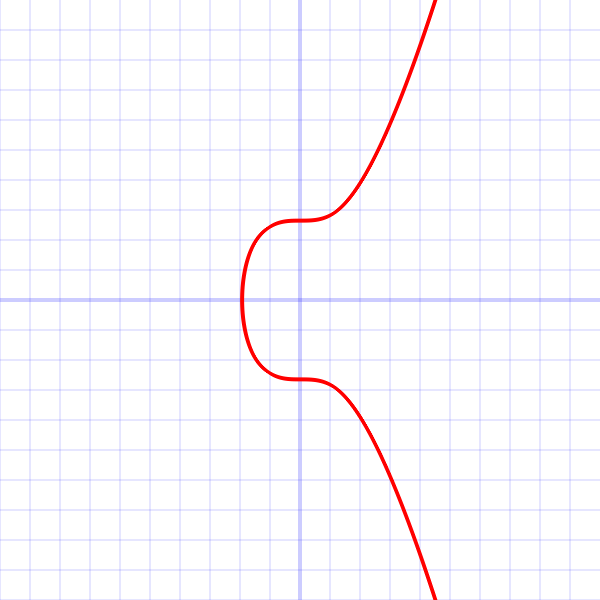
\includegraphics[width=0.5\textwidth]{introduction/images/Secp256k1.png}
	\caption{The \texttt{Secp256k1} plotted over real numbers. Note that the real
	curve is over a field, and thus looks more like a scattering of random points}
	\label{fig:eccbasic}
\end{figure}

The elliptic curve used can hold different parameters that defines it, certain
elliptic curves are standardized and have their own names. The curve used in
Bitcoin is named \texttt{Secp256k1}.\cite{Secp256k1_def}\cite{antonopoulos_2017}

The typical curve used in Elliptic curve cryptography is on the form
$y^2=x^3+ax+b$. The \texttt{Secp256k1} is defined with $a=0$ and $b=7$, making
the full \texttt{Secp256k1} equation: $y^2=x^3+7$. Which is plotted in figure
\ref*{fig:eccbasic}. For more in depth on elliptic curve cryptography see
section \ref{ecdsa}

%Mastering bitcoin
\Subsection{Blocks and the blockchain}
A block is fairly simple to understand, it is simply a datatype or structure
that holds information about itself, all the transactions that can fit and the
previous block in the chain (more on that in a bit). Because every block holds
information about the previous block you can follow all blocks backwards in time
all the way back to the original, also called the genesis block.\cite{genesis}
This is what is referred to as the blockchain.

A block could be added to the chain by anyone in the world. However it will only
be accepted if it has sufficient proof-of-work, and this is the key to how
consensus is reached in the network.\cite{antonopoulos_2017}

\begin{figure}[H]
	\centering
	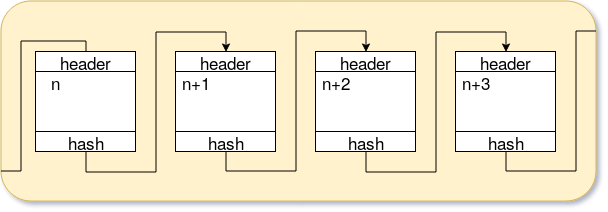
\includegraphics[width=0.5\textwidth]{introduction/images/blockchain.png}
	\caption{A basic overview of a blockchain}
	\label{fig:blockchain}
\end{figure}

\Subsubsection{Block-header}
Each block has a section of data called a header. The header contains meta-data 
about the block itself such as the version number, the id of the previous block 
in the chain, a timestamp of when the block was mined, the merkle root\footnote{See glossary} of 
all transactions (serves as proof of what transactions was included in the block) 
and a 32-bit field called nonce. 

The size of the header is always 80-bytes, a blocks id\footnote{Block id and 
block hash refers to the same thing. The terms might be mixed throughout the report.} 
is equal to the hash of its header. For example the genesis block in the 
Bitcoin blockchain has the id:

\texttt{000000000019d6689c085ae165831e934ff763ae46a2a6c172b3f1b60a8ce26f}

Something that you will find with all block-ids is that they always have leading zeroes. 
This is a side-effect  caused by mining and proof-of-work as explained in section \ref{intro-proof}.

%The section on SHA256 can be improved
\Subsection{Proof-of-work}\label{intro-proof}
Proof-of-work is, just like digital signatures, based in cryptographic
mathematics. Before we go on, you first need to understand what a hashing
algorithm does, the hashing algorithm used in Bitcoin is called \texttt{SHA256}.
\texttt{SHA256} takes in data of any size and produces a sort of finger print
of 256 bits.

For example the \texttt{SHA256} of the text ''cool'':

\fbox{\begin{minipage}{\textwidth}
	\texttt{echo "cool" | openssl sha256}
\end{minipage}}

Produces:

\fbox{\begin{minipage}{\textwidth}
		\texttt{27c16ce7e3861da034af1bb356d6a4f38cb84fa65d51fa62f69727143b4c6b60}
\end{minipage}}

The text produced is actually bytes represented in a hexadecimal number system,
in fact the entire string can be considered to be a very large number. Just like
with the digital signature there is no known viable way that can take a hash and
find what the original data that produced it was.

There is a term in Bitcoin called mining difficulty, or just difficulty. This
is a large number, 256 bits to be exact. When you want to add a new block to
the chain you have to do something called mining, this is a process where you
change the nonce-bits in the block-header until the hash of the blockheader (Think
of this as a number) is less than the target difficulty. The term hashpower refers
to how many times the machine you are using to mine blocks can test a certain
combination of variables per second, or H/s (Hashes per second).

The difficulty of mining a block is adjusted about every 2 weeks (every 2016th block to be exact). The difficulty
is calculated by each individual node whenever the block count is a multiple of 2016, the nodes go by the timestamps in the blocks, and should thus all reach the same conclusion. The new calculated difficulty is the one all the next 2016 blocks have to reach.\cite{antonopoulos_2017}

The accepted order of transactions is the order going backwards from the latest
block on the longest chain. The longest chain is always the one that the majority
is mining towards. What it basically
means is that as long as you trust 51\% of the participants in the network you
can also trust that the order of transactions is correct.\footnote{This is a simplification, but still holds true} This mechanism
prevents things like double spending the same money and holds a property called
emergent consensus, which means that eventually the entire network will agree
on the order of transactions.

In figure \ref{fig:blockchain2} is a diagram showing the longest chain, meaning
the chain with most proof of work. The block in green is the latest block on
that chain. The yellow block is what is known as a stale block, a block that is
part of the chain but not part of the longest chain of blocks. Transactions in
a stale block are not considered valid, and eventually they can be pruned
(deleted) because they do not effect the future in any way. A stale block occurs
if a new block is found in different parts of the network at almost the same
time. Then the network will be split, each node tries to find the next block on
the chain of whatever block they received first. In the case shown below the
chain on the left ''won'' and the green block is now the longest chain.

The red block in figure \ref{fig:blockchain2} is what is known as an orphan
block, that is, it has no known parent in the chain. This can happen if someone
mines a block that is malformed or when building the chain for a new node and
the blocks are received out of order.

\begin{figure}[H]
	\centering
	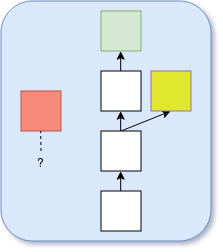
\includegraphics[width=0.2\textwidth]{introduction/images/more_blockchain.png}
	\caption{A diagram showing the longest chain, The green block is the latest
	block on the longest chain. The red block is a an orphan block, the yellow
	block is a stale block}
	\label{fig:blockchain2}
\end{figure}


\Subsection{Software}
Just like how you can use regular money without knowing the underlying process
and technology of banking systems for example, you can use Bitcoin without
knowing the details of how it works. There is plenty of software that handles
wallets, transactions etc for you.

%Removed for now
%A good example is mycelium wallet for Android.

\Subsection{Programmable transactions}
Another feature that Bitcoin has, which makes it very versatile, is that transactions are programmable.
As mentioned earlier the most
common transaction is sending the money to someones public key. What really
goes on here is that the person who wants to spend whatever money was sent to
them has to prove programmaticlly that they own the private key related to that
public key.

This is not the only type of transaction possible, Bitcoin has its own little
programming language called \texttt{Script}. Any type of transaction that can
be described in script is possible as a transaction. This is the basis for atomic swaps, payment channels and lightning network, which will be discussed in the following sections


%might be cut form the full report

%https://wstein.org/edu/2007/spring/ent/ent-html/node89.html
\Section{Elliptic-curve cryptography \& ECDSA}\label{ecdsa}
As covered in the introduction, Elliptic-curve cryptography (\textbf{ECC}) and ECDSA 
is a fundamental building block of bitcoin. Elliptic curve cryptography relies on 
intractability of calculating the discrete logarithm of a elliptic curve element with 
respect to a publicly known base point. Or put another way: It is easy to calculate 
elliptic curve multiplication with multiplicand $n$. But calculating $n$ from the 
resulting point is considered infeasible with sufficiently large curves and multiplicands.

%Not sure about the field
An elliptic curve is defined by the equation $Y^2=x^3+ax+b$ and six domain parameters 
$E(p,a,b,G,n,h)$. $\textbf{p}$ is the field that the curve is defined over, this 
is usually a very large prime number. The curve being defined over a field simply 
means that the points on the curve fall within $[0, p]$ rather than within the 
real numbers $\mathbb{R}$. In other words the curve is defined over the field 
$\mathbb{F}_{p}$. $\textbf{a}$ and $\textbf{b}$ are whatever number you put into 
the equation. $\textbf{G}$ is the generator point, that is the point on the curve 
that will be used in point multiplication later. $\textbf{n}$ is the order of G. What 
that means is that $n$ is the largest number that $G$ can be multiplied by before 
a point at infinity is produced. $n$ pretty much tells you the limit on how points 
on the curve that can be generated from $G$. $\textbf{h}$ is the co-factor of the 
curve. It can be calculated as follows: $h=\frac{1}{n}|(E(\mathbb{F}_{p})|$, where 
$|(E(\mathbb{F}_{p})|$ is the order/cardinality of the group of points possible on 
the curve over field $\mathbb{F}_{p}$. $n$ is derived from $G$, $G$ and $p$ should 
be chosen in such a way that $h \leq 4$, preferably $h=1$.

These domain parameters can be chosen manually or you can use predefined parameters. 
Elliptic curves that used predefined domain parameters are called named-curves. 
The named curve used by Bitcoin is called \texttt{Secp256k1}

\Subsection{Secp256k1}
\texttt{Secp256k1} is defined with the following domain parameters (hexadecimal):\\\\
$p=\texttt{FFFFFFFF FFFFFFFF FFFFFFFF FFFFFFFF FFFFFFFF FFFFFFFF FFFFFFFE FFFFFC2F}$\\
or alternatively:\\
$p=2^{256}-2^{32}-2^{9}-2^{8}-2^{7}-2^{6}-2^{4}-1$

$a=0$\\
$b=7$

$G=(\texttt{79BE667E F9DCBBAC 55A06295 CE870B07 029BFCDB 2DCE28D9 59F2815B 16F81798},\\ \null\qquad\:\:\: 
\texttt{483ADA77 26A3C465 5DA4FBFC 0E1108A8 FD17B448 A6855419 9C47D08F FB10D4B8})$


$n=\texttt{FFFFFFFF FFFFFFFF FFFFFFFF FFFFFFFE BAAEDCE6 AF48A03B BFD25E8C D0364141}$
$h=\texttt{1}$

\Subsection{Math on the elliptic curve}
Two mathematical operations needs to be defined to operate on the elliptic curve: 
addition and multiplication

\Subsubsection{Point addition}
Let's say you have to distinct points P and Q that both fall on curve $E(p,a,b,G,n,h)$ 
($Y^2=x^3+ax+b$). 

$$P+Q=R \Rightarrow (X_P, Y_P) + (X_Q, Y_Q) = (X_R, Y_R)$$

$$X_R = \lambda^2-X_P-X_Q$$
$$Y_R = \lambda(x_P-X_R) -Y_P$$

where $\lambda$:

$$\lambda = \frac{Y_Q-Y_P}{X_Q - X_P} \mod p$$

\Subsubsection{Point multiplication}
If P and Q are coincident, meaning that they have the same coordinates the equation 
is slightly different. 

$$P+Q=R \Rightarrow P+P=R \Rightarrow 2P=R$$ 

This could be seen as P being multiplied with scalar 2. Most of the equation is the same 
as with addition, the difference is that:\\
$$\lambda = \frac{(3X^2_P + a)}{(2Y_P)} \mod p$$

\Subsubsection{Faster multiplication with large scalars}
Take $xP=R$ that could be calculated by summing P x times:
$$\sum_{n=1}^{x} P = R$$
This might work fine for smaller numbers but for a very large number, like $x=2^{100}$ it will 
take infeasible amount of time to calculate. Luckily there is a convenient short cut that you 
can take called double and add. 

First remember that: $P+P = 2P \Rightarrow 2P + P = 3P \Rightarrow 4P = 2(2P) \Rightarrow 8P = 2(2(2P))$

Lets say $x=200$ in binary terms this could be written as $x=128+64+8$ or $x=2^7+2^6+2^3$ 
thus $200P=R$ could be written as 
$$2^7P+2^6P+2^3P=R$$ 
which could be shorten to: 
$$2(2(2(2(2(2(2P)))))) + 2(2(2(2(2(2P))))) + 2(2(2P))$$ 
which looks cumbersome but now instead of 200 calculations you only have to do 18.


\Subsection{Private and public key}
Just as \texttt{RSA} cryptography, ECC relies on public-private key encryption and signatures. 
The public key can be shared freely to everyone, while the private key should, as the name implies, 
be kept private. Each unique private key has a corresponding public key, through mathematics it 
can be proven that someone holds the private key paired with a certain public key, without actually 
revealing the private key. 

In ECC \textbf{a private key is a really large number}. Imagine you have curve $E(p,a,b,G,n,h)$ 
and you want to generate a brand new private key k. k could be any number between 0 and $n$. Any 
$k > n$ will produce the exact same public key so that will not work. \textbf{A public key in ECC is 
represented by a point in 2D space}, more specifically a point that falls on the curve. To generate a 
public key P from a private key k you perform $kG = P$ as described in the section above.

\Subsubsection{Compressed key}
\begin{wrapfigure}{r}{0.3\textwidth}
	\begin{center}
		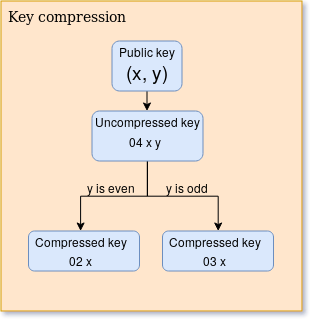
\includegraphics[width=0.4\textwidth]{background/images/key_compression.png}
	\end{center}
	\vspace{-8mm}
	\caption{How to compress the public key in ecc}
\end{wrapfigure}

The public key is quite large, with two 256-bit numbers representing coordinates. But there is a 
clever trick we can use to compress the size of the key. Take the \texttt{Secp256k1} curve for 
example ($Y^2=x^3+ax+b$). It is mirrored around the x-axis, meaning that for each x value there 
are two possible y values. Thus a public key can be represented by only it's x value plus a 
prefix telling you which resulting y-value to choose. 

Note that because y and x is over $\mathbb{F}_{p}$ there is no negative value, instead the y 
value is referred to as even or odd. 

\Subsection{ECDSA}
The main usage of ECC in cryptocurrency is for proving ownership of coins. The proof relies 
on elliptic curve mathematics like before. Lets say \textbf{Alice} has a message $m$ and want 
to send it to \textbf{Bob} and also prove that the message came from her. First of let's 
establish some variables: $k_A$ is the private key belonging to Alice, from that private 
key $P_A$ was generated (The public key), that Bob knows about. 

\Subsubsection{Signing}
First calculate the hash of the message:
$$e=HASH(m)$$
If $e$ has a bit-length (numbers in binary representation) that is longer than the bit-length 
of order $n$ of the curve used. $e$ has to be trimmed down so that the bit-lenghts match

Select a cryptographically-secure random number $z$ that falls in the range $[1, n-1]$ and 
calculate a new curve point: $(x_1, y_1) = z \times G$

Calculate $r$ and $s$ such that: $r = (x_1 \mod n)$ and $s = (z^{-1} (e + r \times k_A) \mod n)$. 
if either $r$ or $s$ ends up being 0, generate a new $z$ and try again.

The signature will be the point $(r, s) = S_A$.

\Subsubsection{Signature validation}
If \textbf{Bob} wants to verify that it was actually \textbf{Alice} that signed the message $m$. 
He first has to do a sanity check on the signature $S_A$ to make sure that it is a valid point on 
the curve and that $s$ and $r$ is within the range $[1, n-1]$ etc... 

Calculate the hash $e$ of $m$ the same way as it was done during the signing process. Calculate 
$$w=(s^{-1} \mod n)$$ and $$u_1 = (ew \mod n)$$ $$u_2 = (rw \mod n)$$

From $u_1$ and $u_2$ calculate the point $(x_1, y_1) = u_1 \times G + u_2 \times S_A$ 

The signature is valid if and only if $r = x_1 \mod n$

\Section{Script}

Script is the name of the programming language used in Bitcoin and its derivatives. It was not used to write the Bitcoin implementation but rather it is what makes transactions in Bitcoin so versatile. This section however will not focus on where or how Bitcoin uses Script, but rather on how Script itself functions.

Script is a forth-like stack based language that is not turing-complete.\cite{script_wiki}\cite{antonopoulos_2017} Turing-completeness means that a language can do anything that the imaginary turing-machine could do, in other words it basically means is that the language can do any mathematically sound operation. Script is \textbf{NOT} turing-complete on purpose, a good example is loops, in most languages there is some sort of structure that allows for a piece of code being executed repeatedly. In Scipt this is strictly disallowed, as it has neither for-loops or while-loops. This means that any given script will execute within a well defined deterministic time-span, and can never go on forever.

As mentioned earlier. Script is a stack-based language. That means that as the language executes it uses a stack to store data and variables. Do not confuse the term with the heap and stack from regular programming language discourse. In script there is no heap, instead the stack is the only form of memory, and it acts just as you would expect from a stack, to add a value you have to push it to the stack and to read a value you have to pop it from the stack.\cite{script_wiki}\cite{antonopoulos_2017}

The language itself is quite basic. It relies on operation codes (op codes) the size of a single byte. Most operations pop values from the stack, does something with the values, then pushes the result back on the stack. When Script is written out on paper many op codes and values are excluded, because they are implicit. For example: 

\texttt{OP\_PUSHDATA1 4 FFFFFFFF} 

This operation pushes 4 bytes to the stack, the bytes have the hexadecimal value \texttt{FFFFFFFF}. But usually when this operation is written out it is shorten to just:

\texttt{FFFFFFFF} 

\textbf{Whenever a hexadecimal value appears in the code it is implicit that that value is pushed to the stack in the form of bytes}. Here is another program:

\texttt{4 5 OP\_ADD 9 OP\_EQUAL}

This simple program will push 4 and 5 to the stack, \texttt{OP\_ADD}\cite{script_wiki} pops two values from the stack (4 and 5) adds them together and pushes the result back on the stack. Then a 9 is pushed to the stack. \texttt{OP\_EQUAL}\cite{script_wiki} pops two values form the stack and pushes a 1 if they were equal, 0 otherwise. In this case a 1 will be left on the stack as $4 + 5 = 9$. Figure \ref{fig:script} visualizes what happens at each step of execution. There are other cases where the verify op-code is combined with other instructions.
\\
\begin{figure}[H]
	\centering
	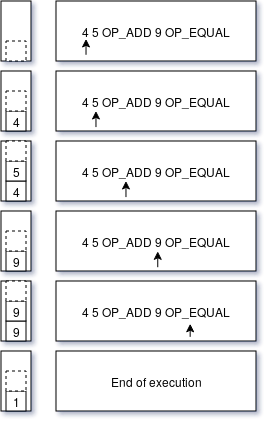
\includegraphics[width=0.4\textwidth]{background/images/script.png}
	\caption{Execution of simple program, to the left is the stack, to the right is the program with execution pointer}
	\label{fig:script}
\end{figure}

\Subsection{Complex operations}

There are some operations in Script with slightly higher complexity, which do not act like the others. One of them is \texttt{OP\_VERIFY}, this will perform a verify check on the script. It will pop one value from the stack, and if that value equates to false execution will end immidietly and the entire script will be marked as invalid (see section \ref{script_valid}).\cite{antonopoulos_2017}\cite{script_wiki} If the value equals true execution will continue where it left off. Some operations are combinations with the verify check, like for example \texttt{OP\_EQUALVERIFY}. This is equal to writing \texttt{OP\_EQUAL OP\_VERIFY}, meaning that it first does an equal check then verifys the result.

\vspace{7mm}
\InsertBoxR{0}{
	\footnotesize\setlength\fboxsep{10pt}\setlength\fboxrule{1pt}
	\fcolorbox{IndianRed3}{SlateGray1}{\begin{minipage}{2.1in}
			\subsection*{Bug in Script}
			An interesting bit of trivia is that there is a bug in the language implementation. More specifically with the operation \texttt{OP\_CHECKMULTISIG}. The bug makes it so this operation pops one more value from the stack than it is supposed to. This was not discovered until the network had been running for a while. It can't be easily fixed as it is now a part of the consensus rules. All implementations of Bitcoin node has to implement the bugged version of this op code otherwise consensus on the validity of transactions will break.
			A fix to this bug would require a hardfok, see section \ref{soft_hard_fork}, so far it has not been done as it is considered to be not worth the time and effort.
	\end{minipage}}
}[9]

There are several operations for checking signatures. These are not so complex in terms of what they do in the script. Their implementation is quite complex however. They rely on outside information that is not present in the script to check the validity of a signature.\cite{script_wiki}\cite{antonopoulos_2017} The two most used are \texttt{OP\_CHECKSIG} and \texttt{OP\_CHECKMULTISIG}. These will not be covered in full in this section as they are more related to transactions so see section \ref{transactions} for a full explanation. 

\Subsection{Valid and invalid scripts}\label{script_valid}
At the end of execution a script is marked as either \\valid or invalid. A script is invalid for the following \\reasons\cite{antonopoulos_2017}:

\begin{itemize}
	\item The stack is empty
	\item There are more than one values on the stack
	\item The only value on the stack equates to false
	\item A VERIFY check fails sometime during execution.
\end{itemize}

A script is valid if and only if there is one value on the stack, and it is not equal to false.

%https://en.bitcoin.it/wiki/Transaction
%mastering bitcoin
\Section{Transactions}\label{transactions}
Transactions in Bitcoin are not as straight forward as you might expect a transaction to be. A transaction contains a list of inputs and a list of outputs as well as some metadata like version number and lock-time.\cite{bitcoin_core_tx}\cite{antonopoulos_2017}

\begin{figure}[H]
	\centering
	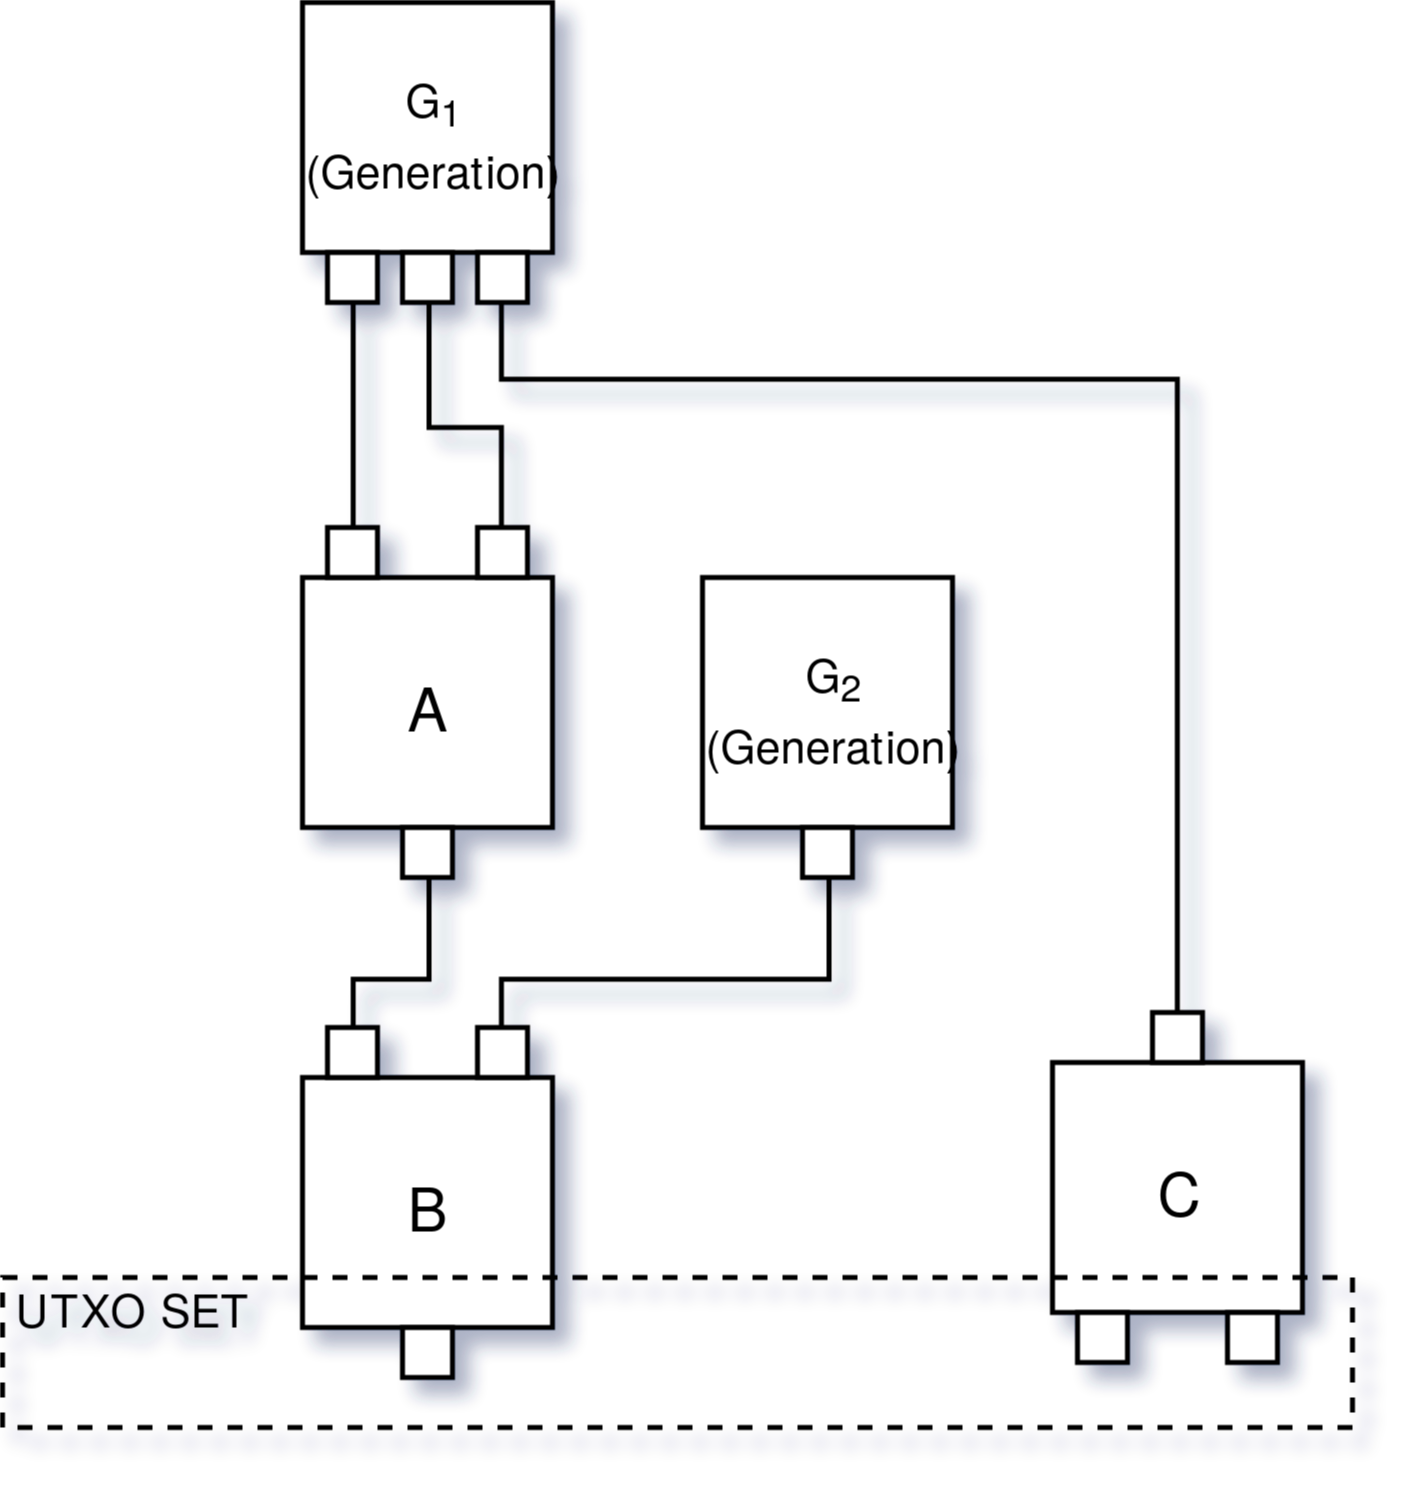
\includegraphics[width=0.75\textwidth]{background/images/transaction_diagram.png}
	\caption{4 example transactions and how inputs are connected to outputs}
	\label{fig:transaction_input_output}
\end{figure}

In simplified terms an output could be seen as the destination of a transaction, in other words it says how much and to whom the transaction is sent to. An input is a reference to a previous output. The inputs take the money from the outputs they reference and that money is used to fund the new outputs.\cite{antonopoulos_2017}\cite{bitcoin_core_tx}

The inputs and outputs is where Script comes into the picture. Both outputs and inputs contains an incomplete script, together however they complete the script. The script in an output could be seen as a challenge, and the script in the input is the response. When a transaction is tested for validity the input script is appended to the script in the output and is executed. If the script comes out as valid the transaction is also valid.\cite{antonopoulos_2017}\cite{bitcoin_core_tx} Here is a basic example: Let's say Alice wants to send a transaction to whoever can answer the equation $4+3$. Her transaction output would contain the script:

\texttt{4 3 OP\_ADD OP\_EQUALS}

If this is executed as is it is invalid. But let's say Bob knows the answer to the equation he can then create a new transaction where the input contains the script: 

\texttt{7} 

Just as before this script is not valid by itself. But then the transaction is checked for validity the input will be appended to the start of the output script forming the following: 

\texttt{7 4 3 OP\_ADD OP\_EQUALS}

Which is a valid script, thus Bobs new transaction is also valid and he may spend the money as he see fits. 

Obviously most transactions on the Bitcoin blockchain are not this simple. The most common form of transaction contains a script called P2PKH which stands for Pay to public key hash. Before we can go into details on this one however we first need to know about how signatures and sighash work in script and transactions.

\Subsection{Signatures and sighash}
Section \ref{ecdsa} covers public keys and signatures in depth.

Perhaps the most important operation in script is the \texttt{OP\_CHECKSIG} operation and its cousins. \texttt{OP\_CHECKSIG} pops two values from the stack, if the script is correctly implemented these two values should be the public key and a signature created with the private key that correlates with mentioned public key

The question is: what is signed when the signature is created? Broadly speaking it is the hash of the transaction that is trying to spend the output, this is not entirely accurate however.\cite{antonopoulos_2017} Appended to the signature that is a flag called \textbf{sighash} (Signature hash). The value of sighash tells the script interpreter what hash was signed during the creation of the signature.\cite{bitcoin_core_sighash} There are 4 types of sighash implemented:

\Subsubsection{SIGHASH\_ALL}
This can be considered the default sighash, if it is not stated otherwise it can safely be assumed that this type was used. This simply means that the entire transaction is signed with all outputs and all other inputs.

\Subsubsection{SIGHASH\_NONE}
This one signs the transaction but without the outputs, it could be thought of as ''I don't care where the money goes''.

\Subsubsection{SIGHASH\_SINGLE}
All outputs are removed except the output with the same index as the input that is being signed, then that transaction is signed.
This could be thought of as ''I dont care about any other outputs to this transaction as long as this one remains as is''.

\Subsubsection{SIGHASH\_ANYONECANPAY}
Signs the transaction with all the outputs but none of the other inputs. This basically means ''The money has to go here, but I don't care if someone else want to fund this transaction also''

%\Subsubsection{More detailed process}
%On the next page the entire signing process for SIGHASH\_ALL is detailed. This is how it is performed in the actual implementation:
%\newpage
%\centerline{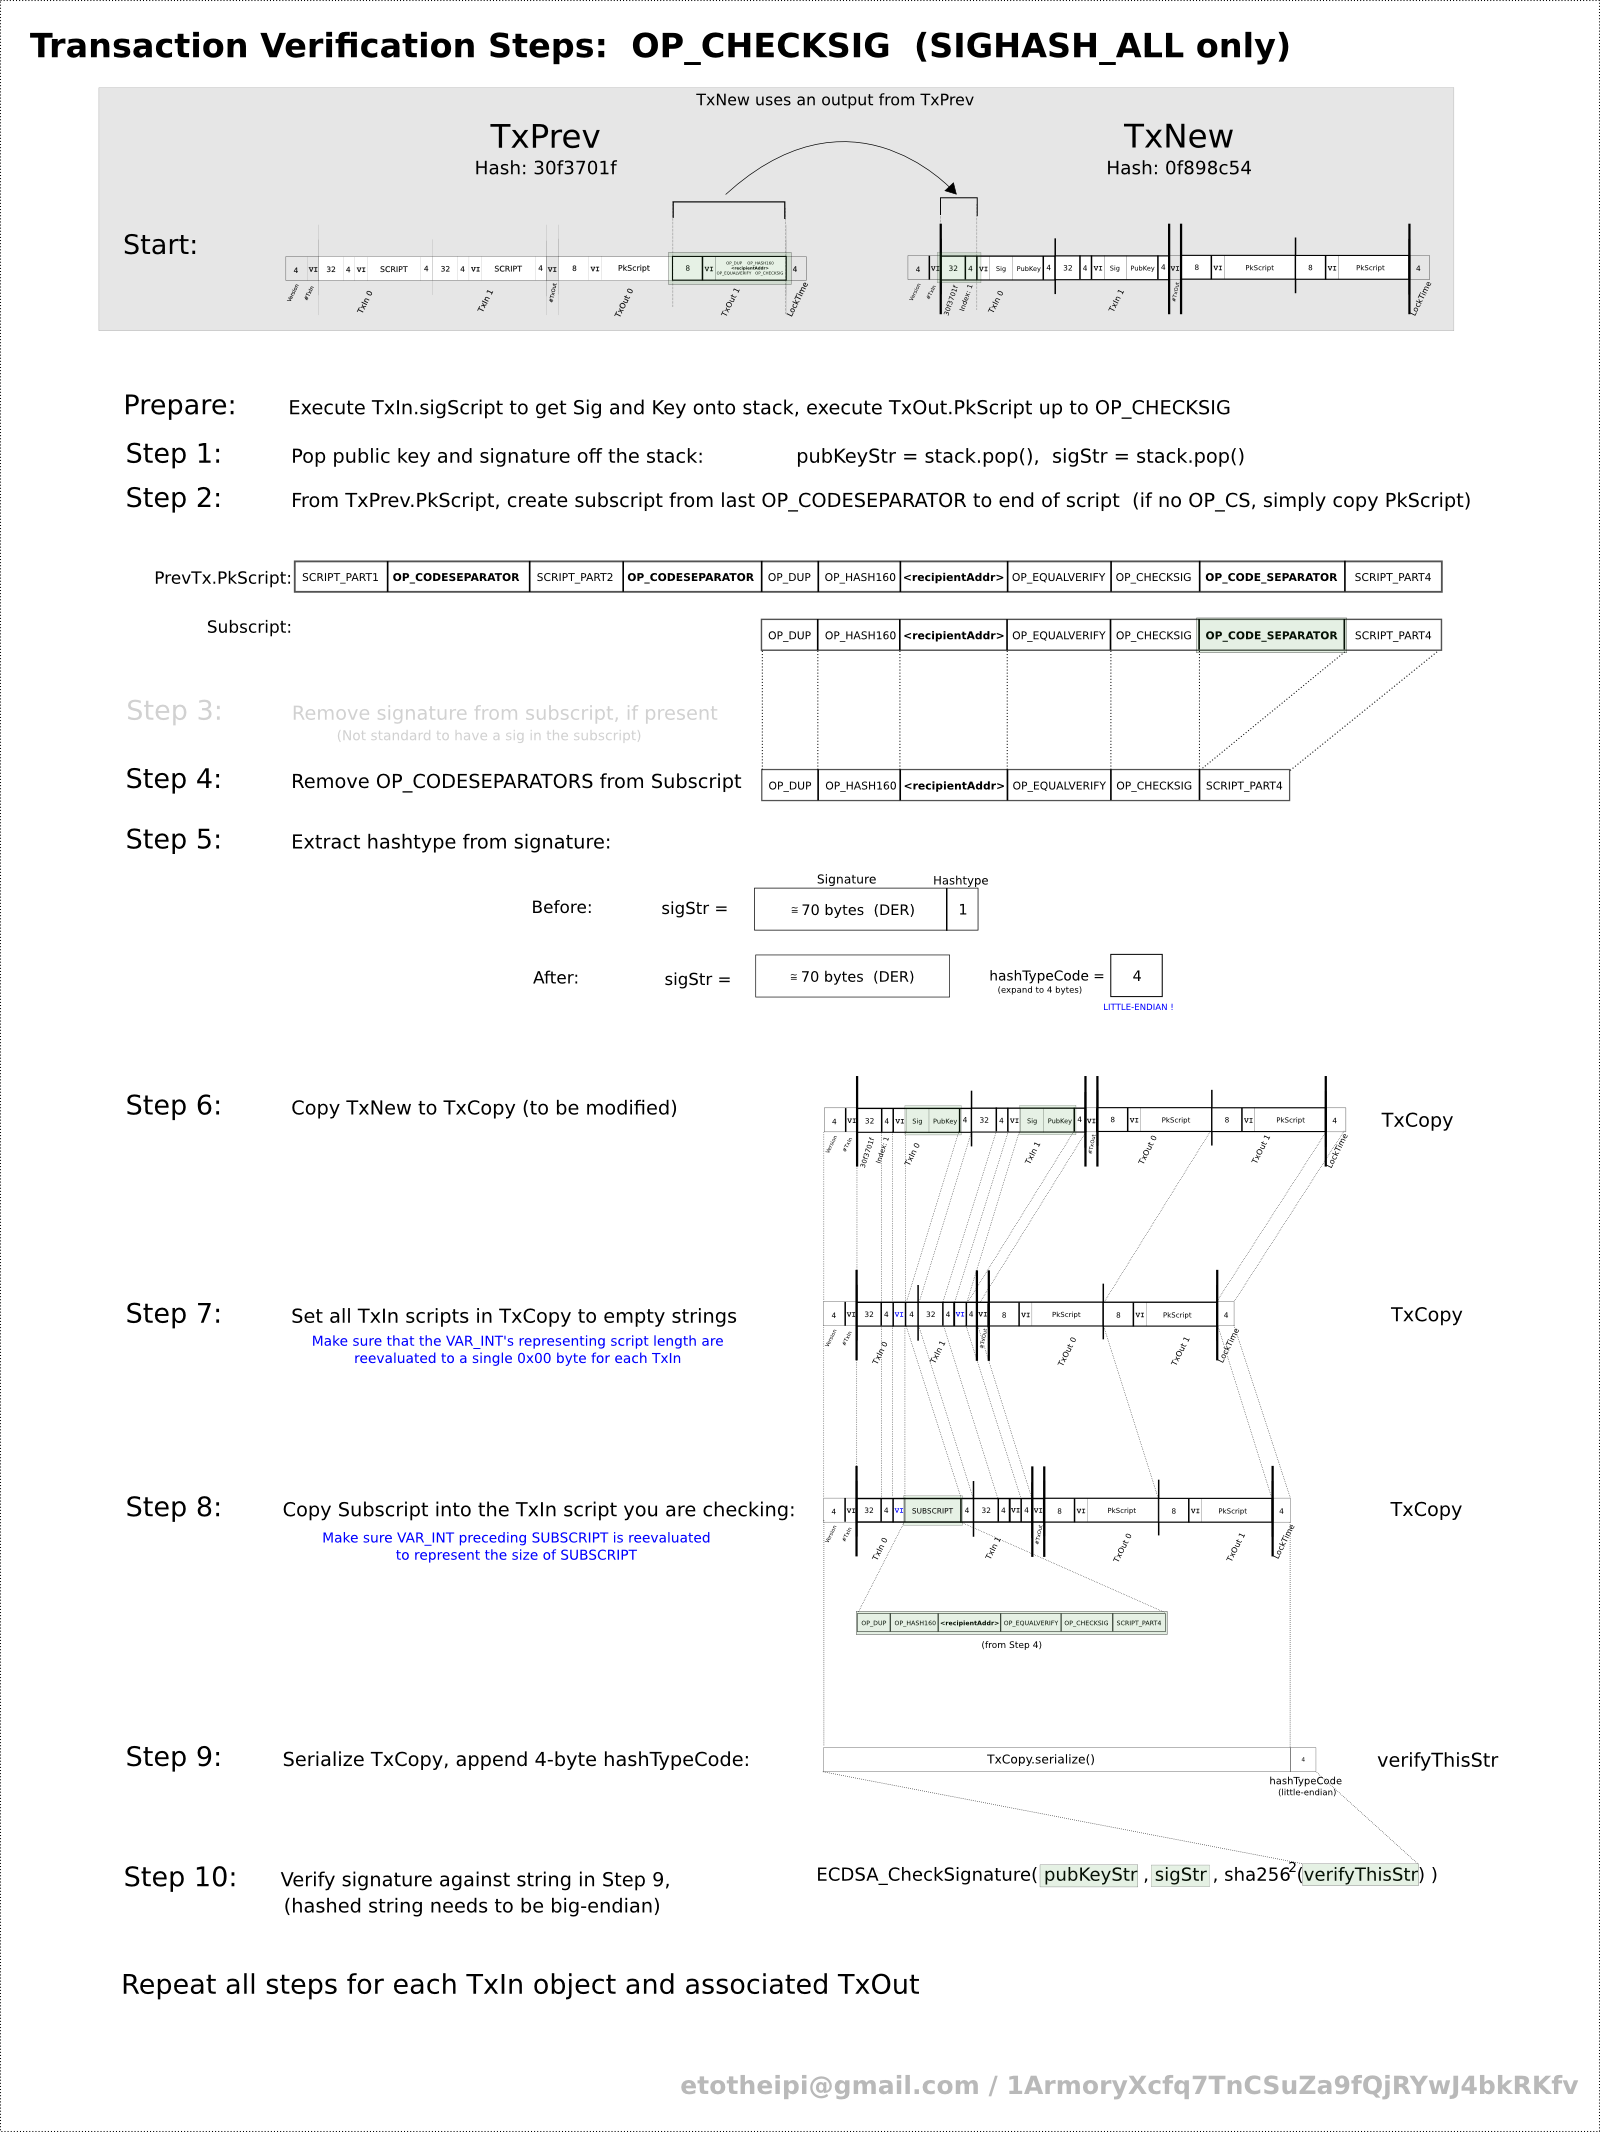
\includegraphics[width=1.35\textwidth]{background/images/checksig_in_detail.png}}
%\newpage

\Subsection{Pay to public key hash (P2PKH)}\label{p2pkh}
P2PKH is as mentioned the most common form of transaction.\cite{antonopoulos_2017} This transaction can be thought of as paying to somebodies address. In other words the output of this transaction contains a script where the one who wants to redeem it must prove that they own the private key which created the public key the address is referring too. This is what the script looks like in the output:

\texttt{OP\_DUP OP\_HASH160 <public key hash> OP\_EQUALVERIFY OP\_CHECKSIG}

As mentioned already executing the script in the output by it self doesn't make any sense, especially now when the very first operation \texttt{OP\_DUP} tries to duplicate the top element in the stack. But at execution the stack will be empty. Anyone wanting to spend this output would construct a transaction with the input script on the following form:

\texttt{<signature> <public key>}

When the input and output is executed together the process goes like this: 
\begin{enumerate}
	\item First the signature and unhashed public key is pushed to the stack.
	\item The public key is duplicated (there are now one signature and two public keys on the stack).
	\item The top public key goes through the HASH160 process making it a hashed public key.
	\item The hashed public key from the output is pushed on the stack, at this point the stack has the following elements (\texttt{<signature>}, \texttt{<public key>}, \texttt{<hashed public key>}, \texttt{<hashed public key>}).
	\item \texttt{OP\_EQUALVERIFY} checks if the top two elements is equal and verifies the result, What basically has been done is is that the script checks if the public key provided in the input script is equal to the hashed public key given in the output script.
	\item At this point the stack has the following elements: (\texttt{<signature>}, \texttt{<public key>}). \texttt{OP\_CHECKSIG} pops these from the stack and checks if the signature is valid.
\end{enumerate}

In the early days of bitcoin you payed directly to public keys instead of hashed public key. The reason the hash part was added at all has to do with extra security. If an exploit is found in elliptic curve cryptography that makes it so someone could calculate the private key from a public key then all unspent outputs would be at risk of being stolen. With the hashed public key the actual public key is not revealed until the output is spent, and then it is too late for it to be stolen. This of course requires that everyone uses a different public key for every transaction, which is the standard today.\cite{bitcoin_core_tx}

\Subsection{Pay to script hash (P2SH)}
Pay to script hash is slightly newer and a bit more complex to understand. Instead of paying to someones address, you pay to a script, this was initially proposed by Gavin Andreasen in 2012.\cite{scripthash} Let's say Alice has partial script S, that can be solved with the partial script K. She can then hash S and get $H_S$. She then creates transaction with an output containing the following script:

\texttt{OP\_HASH160 <$H_S$> OP\_EQUAL}

If Bob wants to redeem this transaction he first has to know the script and how to solve it. This is how the transaction input would look like: 

\texttt{K <S>}

The execution of the combined input output script is not straight forward as most scripts are. This is the process:
\begin{enumerate}
	\item The K part of the script is executed as usual. This pushes or does whatever it needs to do to make K + S a valid script.
	\item The partial script S is pushed to the stack in the form of bytes.
	\item This is where the execution takes a strange and not so intuitive path, as you will see. First the script is hashed with the \texttt{OP\_HASH160} operation.
	\item The script hash from the output is pushed on the stack.
	\item OP\_EQUAL checks if the top two items on the stack are equal. If they are it means that the script S provided in the input is the correct script.
	\item Unique to P2SH, the execution goes back to the original script S that was pushed to the stack in stage 2. And executes it together with whatever K pushed to the stack. This script also has to be valid.\cite{scripthash} 
\end{enumerate}

If all stages are executed without error the redeeming transaction is valid. 

P2SH was developed to resolve the difficulties in making complex transaction scripts and make them as simple as paying to an address. What P2SH basically means is ''pay to a script matching this hash, a script that will be presented later when this output is spent''\cite{antonopoulos_2017}\cite{scripthash}

\Subsection{Timelock and sequence}
Since the start of bitcoin; transactions has had two fields in them called \textbf{nTimelock} and \textbf{nSequence}. The timelock variable stopped a transaction from being  included in a block until a certain unix-timestamp or a certain blockheight\footnote{Blockheight is the number of blocks on the current chain} had passed. The sequence field is part of each input into a transaction, it's original purpose was to give users a mechanism for updating a transaction that were still in the transaction-pool. Miners were supposed to include the transaction version with highest sequence number, this however was unenforceable, as there is no way of knowing which transactions were in the transaction-pool of the miner at the time of block creation. So nSequence became mostly defunct and saw little use.

To make timelocks more versatile and more easily enforceable Peter Todd proposed an addition to Script, a new op-code that verifies that the correct timestamp is set, \\\texttt{OP\_CHECKTIMELOCKVERIFY}.

As timelocks only allows for absolute wait time, like for example: ''this transaction can only be spent after \texttt{10th June 2019}''. Mark Friedenbach et al. proposed in 2015 to add an additonal op code to Script that can check for relative time passage as well, \texttt{OP\_CHECKSEQUENCEVERIFY}.

\Subsubsection{OP\_CHECKTIMELOCKVERIFY}
There is an operation in Script called \texttt{OP\_CHECKTIMELOCKVERIFY}, what it does is that it compares the timestamp or blockheight that is on the stack and compares it to the timestamp that is in the transaction trying to spend the output that this op code is part of.\cite{antonopoulos_2017}\cite{checklocktime}\cite{script_wiki}\cite{bitcoin_core_tx}

\Subsubsection{OP\_CHECKSEQUENCEVERIFY}
\texttt{OP\_CHECKSEQUENCEVERIFY} is a lot like the previous one except it it deals with relative time. 

Let's say you have two transactions transaction $T_A$ and transaction $T_B$, $T_A$ is included in a block on the blockchain. If $T_B$ tries to spend one of $T_A$ outputs and has that specific input marked with a  sequence of 10. It means that $T_B$ can't be included in the block chain until $T_A$ is at least 10 blocks deep in the blockchain.\cite{antonopoulos_2017}\cite{checksequence}\cite{script_wiki}\cite{bitcoin_core_tx}

\texttt{OP\_CHECKSEQUENCEVERIFY} enforces this in the output. If $T_A$ has \texttt{10 OP\_CHECKSEQUENCEVERIFY}, then if $T_B$ tries to spend that output it has to be at least 10 blocks deep.


\Section{Segregated Witness}\label{segwit}
Segregated witness (sometimes called just segwit) is a relatively recent addition to bitcoin. A witness in cryptography is a proof of knowledge, for example a signature that acts as proof that whoever created the signature knows the private key that created a certain public key. A signature can also act as proof that the signer knew the content of whatever data that was signed.\cite{antonopoulos_2017}\cite{ecc_def}

\textbf{In bitcoin the script in each input is the witness}, and segregated witness means that the witness part of the transaction is separated from the transaction. The witness is still sent with the transaction when broadcasting, but it is no longer part of the transaction structure.\cite{antonopoulos_2017}\cite{segwitbip}

The reason for this change has to do with malleability. If a transaction still has the witness data it can be manipulated in millions of ways, and all these manipulated versions will all be valid. Let's look at an example, If a transaction has the following input script:

\texttt{<signature> <public key>}

A malicious actor could manipulate the script like this for example:

\texttt{1 OP\_DROP <signature> <public key>}

The script is still valid.\footnote{A transaction with that input script would be rejected in current implementation, but it shows the concept of malleability pretty well} Witness manipulation is not a security flaw in terms of monetary loss as the outputs can not be manipulated without breaking the signatures. What is changed however is the txid. The txid is used to identify the transaction, it is the hash of the entire transaction, you could imagine Alice sending money to Bob, Bob manipulates the transaction so that the txid changes, one of the manipulated transactions makes it into a block thus making all other versions, including the original, invalid, Bob got his money but he can now tell Alice that he did not. Alice tries to find her transaction in the blockchain with the txid she had but it can not be found.

Segregated witness was proposed by Eric Lombrozo et al. in December 2015 and activated via a soft fork on \texttt{21st July 2017}\cite{antonopoulos_2017}\cite{segwitbip}, its purpose is to make the Bitcoin network ready for lightning network usage.\cite{segwitbip} Segregated witness is not a necessity for payment channels and lightning network. But it does make it significantly safer.\cite{segwitbip} A great example is the funding of payment channels. The funding transaction requires the signature of both parties to be spent, to prevent a malicious actor from broadcasting the funding transaction and locking both participants money eternally both signs the initial commitment transaction. The commitment transaction of course use the id of txid of the funding transaction as reference. With malleable transactions a malicious actor could modify the funding transaction and broadcast it. The commitment transaction would be useless as its referenced txid does not exist.

As mentioned segwit separates the witness and transaction. This makes it so the witness is no longer part of the txid, making it effectively immutable. The witness data is stored separately to the blockchain and it's byte-size is not counted towards the block size, making it so more transactions could fit in a single block; it does not make the storage requirement any smaller as the witness data still needs to be stored for validation. 

\Section{Payment channels}
A payment channel is a channel where transactions can be exchanged trustlessly on channels other than directly on the blockchain.
This is what is usually referred to as off-chain transactions.
In their most naive form a payment channel can simply be Alice and Bob exchanging promises of future transactions later.
This however is not trustless and any of the parties could later withdraw from the promise without punishment (other than maybe loss of friendship and future trust).

To build a trustless payment channel there are several ways to go about as Script is quite versatile.
The method that will be covered here uses a type of channel \textbf{funding transaction that requires the signature from both parties to spend}, and the channel balance is updated via special commitment transactions that spend the funding output. Each party in the channel has their own version of the commitment transaction. Whenever a commitment transaction is broadcast to the blockchain the channel is closed as the funding transaction can't be spent twice. To update the balance in the channel both parties create new commitment transactions and signs the other parties commitment transaction.\cite{lightningnetwork_2019}\cite{antonopoulos_2017}
Let's take a look at a naive example:

\Subsection{The naive payment channel}
Imagine Alice and Bob wants to open a payment channel between each other. They create a funding transaction and the initial commitment transactions. Let's say they both funded the channel with 1 Bitcoin each. The initial commitment transactions would then have one output paying 1 Bitcoin to Alice and one output paying 1 Bitcoin to Bob, let's call this commit (\textbf{C0}).
The funding transaction is broadcast to the blockchain.

A bit later Alice buys one funny hat from Bob for 0.1 Bitcoins. To complete the transaction they create two new commitment transaction that pays 0.9 Bitcoin to Alice and 1.1 Bitcoin to Bob and signs them for each other, let's call this new commitment (\textbf{C1}). Any number of transactions could be exchanged this way. The channel could be closed by any one broadcasting their commitment transaction. This naive implementation of a payment channel has a fatal flaw however. 

A payment channel needs some safety measures to be safe from malicious actors. The above example lacks a mechanism for preventing old commitment transactions from making their way into the blockchain and still paying the malicious party.. For example after the initial funny hat transaction above (\textbf{C1}) Alice could just broadcast the initial commit transaction (\textbf{C0}) and reclaim the 0.1 Bitcoins she spent. Bob would have no way of preventing this in this naive implementation.

\Subsection{Transaction flow diagrams}
The transactions that are involved in making payment channels grows larger the more features that are added. To make it easier to understand, diagrams are used together with the descriptions. In Figure \ref{fig:anatomy} a basic overview of the diagram-realm transaction is shown. Lines leading from outputs to inputs means that the connected input are spending that output. Note that one output can be connected to several inputs but each input can only be connected to one output, of course an output can only be spent once, this will be clarified later. A question mark (\textbf{?}) in the broadcaster field indicates either that the sender is unknown or that who sends it is irrelevant. 


\begin{figure}[H]
	\centering
	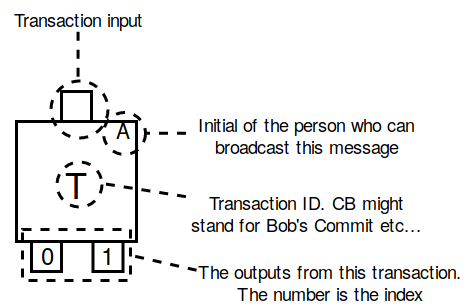
\includegraphics[width=0.5\textwidth]{background/images/tx_anatomy.png}
	\caption{Different parts of a transaction as they appear in diagrams.}
	\label{fig:anatomy}
\end{figure}

\Subsubsection{Payment channel with breach remedy}\label{breach_remedy}
To prevent old transactions from being sent to the blockchain a new mechanism needs to be devised. This can be done via something called revocable delivery and breach remedy (Some times called just revocation).
Instead of both parties holding the same commit. They each get an individual one that differs in its outputs. 

\begin{figure}[H]
	\centering
	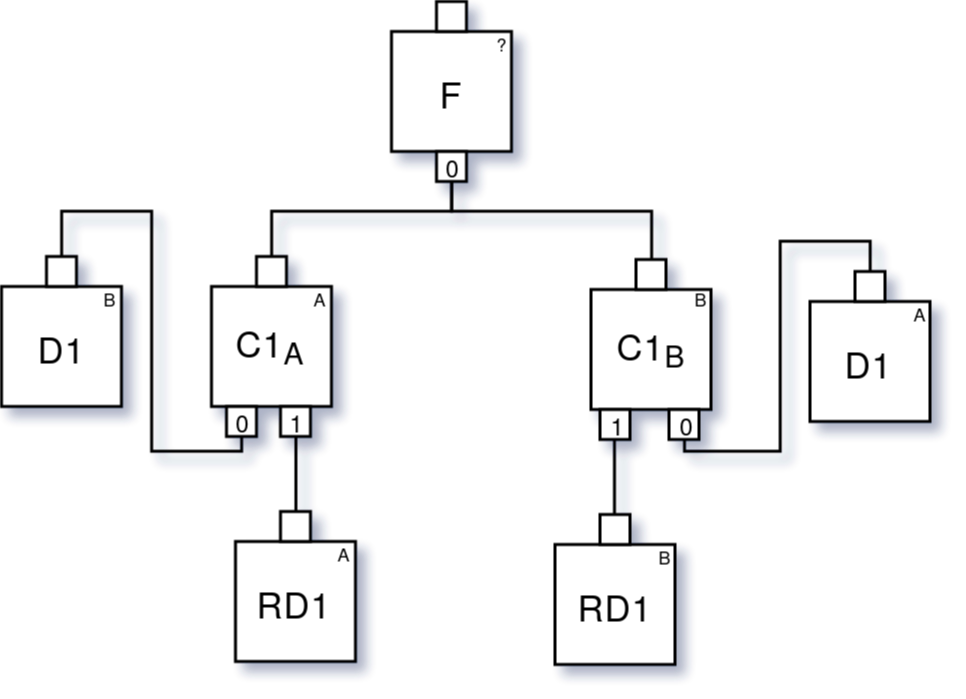
\includegraphics[width=0.6\textwidth]{background/images/payment_channel_pre_breach.png}
	\caption{Payment channel, with commits using revocable delivery mechanism}
	\label{fig:pre-breach}
\end{figure}

Figure \ref{fig:pre-breach} shows how the payment channel appears after the first commitment transactions has been made. Let's say the channel is between Alice (A) and Bob (B) and the balance in the channel is 0.5 BTC for Alice and 0.5 BTC for Bob. 

Let us take a look at the left side of this diagram. \textbf{$C1_{A}$} is the commitment transaction on Alice's side of the channel. As with all commitment transactions it spends the funding transaction. It has two outputs. Output 0 sends 0.5 BTC to Bob completely unencumbered. Output 1 is a bit more complicated however. It pays into a revocable delivery contract worth 0.5 BTC.\footnote{The contract is a script, and it is payed to via P2SH} The contract is constructed with a relative time lock that allows Alice to claim her share of the money after x amount of time (relative to the broadcast time of $C1_{A}$, often described in terms of blocks) or pays to whomever can sign using the pre-generated revocation keys (See section \ref{homomorphism})

D1 is the transaction Bob uses to claim his money in case Alice decides to broadcast her commitment transaction ($C1_{A}$).

RD1 is the transaction that Alice uses to claim her money. The transaction has a relative timelock on it that makes it so it can't be broadcast until x blocks has passed since $C1_{A}$ was included in the blockchain. \textbf{From now on the relative timelock will be 100 blocks in all the following examples}.

The right side is identical, only that the RD1 and D1 relationship is reversed, meaning that Alice can claim her money directly and Bob has to wait. 

If Alice wants to send 0.1 BTC to Bob they need to update the channel with new commitment transactions and then invalidate the old transaction. The transaction diagram will now look like figure \ref{fig:pc-update}

\begin{figure}[H]
	\centering
	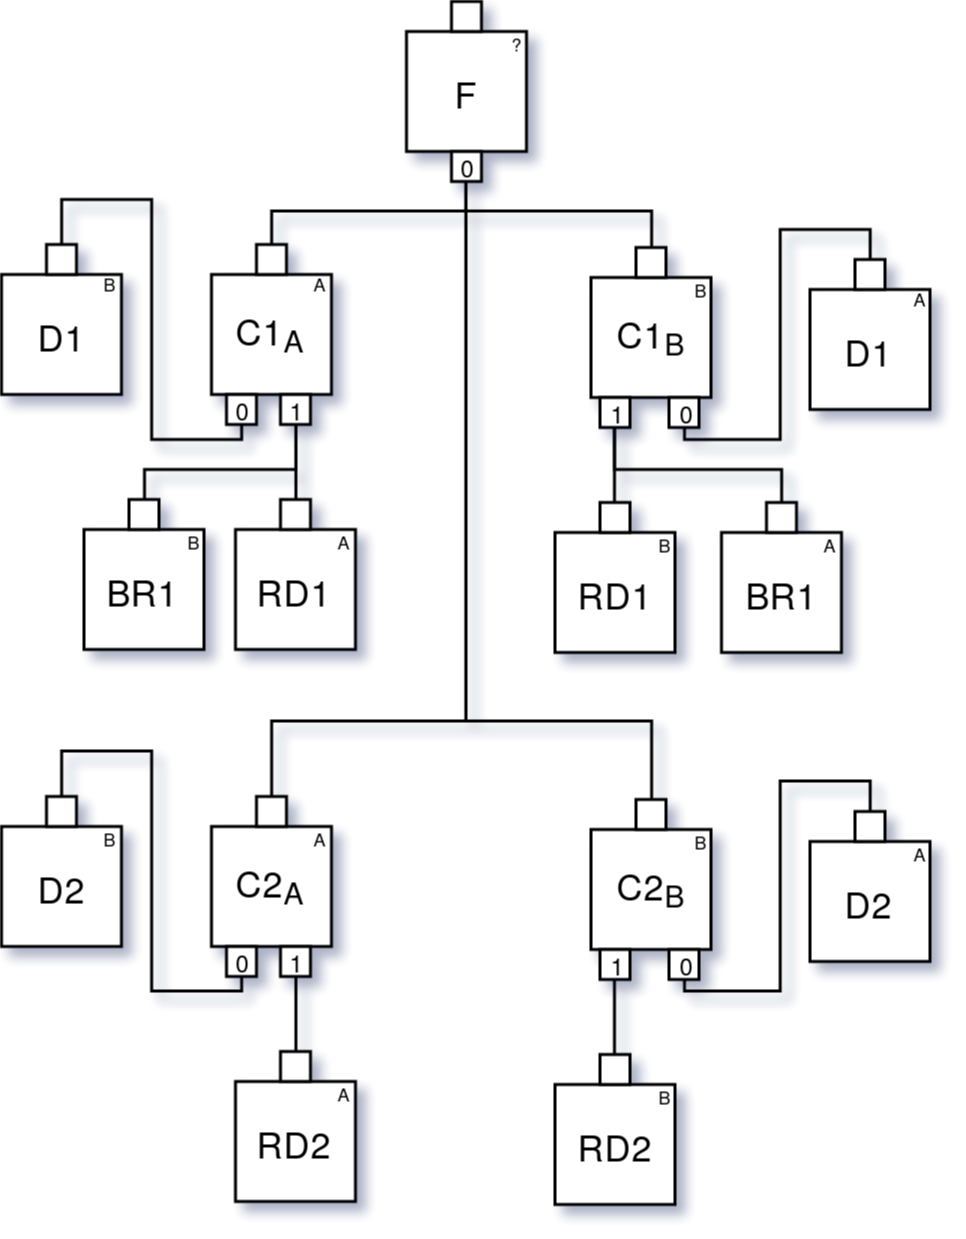
\includegraphics[width=0.65\textwidth]{background/images/payment_channel_updated.png}
	\caption{Updated payment channel, with breach remedies for old commitment transactions}
	\label{fig:pc-update}
\end{figure}

Figure \ref{fig:pc-update} shows the state of the channel after the new commitment transactions have been finalized. 
$C2_{A}$ is a lot like the previous commitment transaction with a few changes. The primary change is of course the channel balance, output 0 now has 0.6 BTC as value and output 1 has 0.4 BTC (Because Alice sent 0.1 BTC to Bob).

Another important update to the channel is the breach remedy. BR1 is the breach remedy for the first commitment transaction, its purpose is to prevent old commitment transactions from being broadcast.\cite{lightningnetwork_2019} The breach remedy can be created after Alice has revealed the secret private key she used when creating the revocation key. Of course to prevent a new false breach remedy to be created for $C2_{A}$ Alice uses a new revocation key for all new commitment transactions. If Alice tries to take back her money by broadcasting an old commitment transaction Bob can prevent it by broadcasting the breach remedy, this is possible because of the timelock on Alice's claim being time-locked.\cite{lightningnetwork_2019}

These are the steps taken whenever someone wants to send money in the channel (Under the assumption that commitment n-1 ($C_{n-1}$) was the latest commitment transaction in the channel), Alice is assumed to be the sender:\\\\
%\begin{enumerate}
	\textbf{1.} Both parties create new revocation public keys.\\
	\textbf{2.} Alice creates the commitment on Bob's side ($Cn_{b}$) using the revocation key from the previous step, signs it and sends it to Bob.\\
	\textbf{3.} Bob creates the commitment on Alice's side ($Cn_{a}$) using the revocation key from the previous step, signs it and sends it to Alice.\\
	\textbf{4.} Each party generates their respective Delivery and Revocable delivery transactions (Dn and BRn)\\
	\textbf{5.} Both parties reveal the secret used to create the revocation keys for the previous commitment transactions ($C_{n-1}$)\\
	\textbf{6.} From these revocation keys each party constructs the breach remedy ($BR_{n-1}$) for the previous commitment on the other persons side.\\
%\end{enumerate}

These steps can be repeated however many times until the channel is closed. 


\Subsubsection{Naive payment network}
The current form of our payment channel works very well as long as it is between just two parties. A very helpful feature would be to be able to send money to anyone without having a direct channel between you and that person, in other word the transaction jumps between any number of other channels before reaching it's destination. If we naively use the channel we have constructed in the previous section as is to send money over multiple jumps we would run into the following problem:

Imagine there being 3 people: Alice (A), Bob (B) and Cecil (C). Alice and Bob have a channel between each other and Bob and Cecil have a channel between each other. Making the following graph: A - B - C. Alice wants to send money to Cecil but they have no channel between each other. To solve this Alice asks Bob to promise to send x amount of money to Cecil if Alice sends x amount of money to Bob. In the perfect world Bob would be honest and this system of payment networking would work. In the real world however having to trust every node between you and the destination would cause problems with malicious nodes. There is nothing stopping Bob from taking Alice's money and never sending anything to Cecil. 

The channel has to be extended further to allow multi-hop payments and still retain it's breach remedy feature. This is where Hashed Time Locked Contracts come into the picture. 

\Subsubsection{Payment channels with Hashed Time Locked Contracts}
A new mechanism needs to be added to our payment channel to enforce that multi-hop transactions actually make it all the way to their destination while at the same time still retaining the breach remedy mechanism etc... 

This could be done by adding a third output to the commitment transactions. This new output pays to a hashed time locked contract (\textbf{HTLC}). Before when a payment was made over a payment channel the amount was updated for each output representing a user in the channel. With the HTLC-output the amount sent is represented by the the value of the HTLC-output. 

A channel could be thought of as having three states: regular, unsettled, and settled. The regular state is the one described in previous sections, it's a channel with one set of active commits, the commit will not have any HTLC-outputs. A channel where the latest commits has a HTLC-output is considered unsettled. The unsettled state should only exists while there is uncertainty about whether the multi-hop transaction completed or not. You could say that \textbf{the HTLC-output only exists as a contingency}, if both parties cooperate the channel can return to regular state with the channel balances updated accordingly, if the parties cannot agree or for some reason will not cooperate the channel should be close as soon as possible, as to why we will get to that. A channel reaches a settled state when both parties decides to close the channel, it is done by creating one last pair of commitment transactions but without any revocable deliveries. After a channel is settled no further transactions could be exchanged in it safely as the mechanism for preventing old transactions from being broadcast has been removed, instead the commitment transaction should be broadcast and the channel properly closed.

To understand the HTLC-output you first need to understand the general mechanism that is used to ensure that multi-hop transactions work. 

\begin{figure}[H]
	\centering
	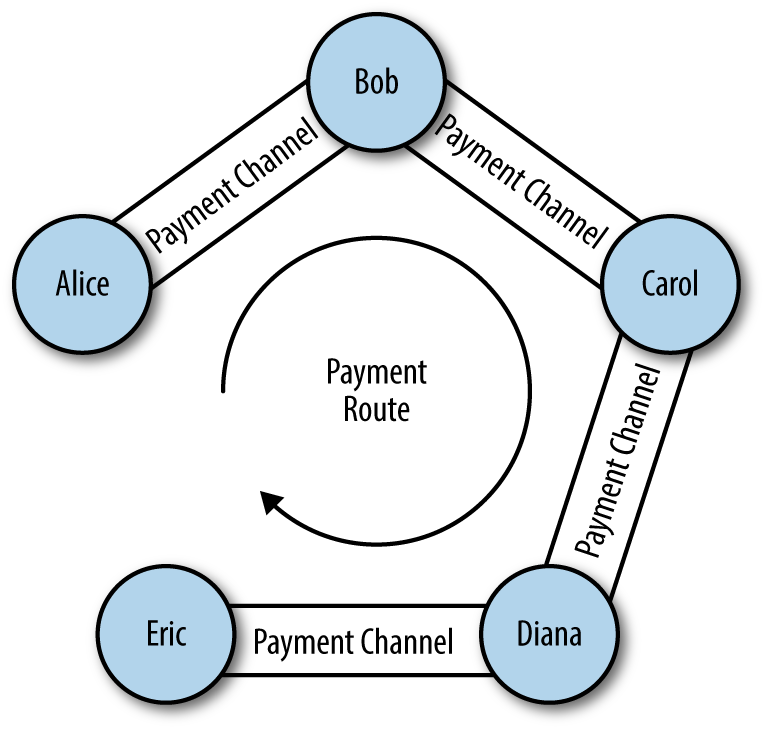
\includegraphics[width=0.55\textwidth]{background/images/pc_route.png}
	\caption{An overview of a network formed by payment channels}
	\label{fig:pc-route}
\end{figure}








\chapter{Atomic swaps}

\Section{On-chain Atomic swaps}
Onchain atomic swaps is a method where two parties can exchange cryptocurrencies between different chains in an atomic way, in this case it means that none of the parties can cheat the other and no matter what state in the exchange-process the swap is either completed or reversed entirely, to the pre-exchange state. The onchain distinction comes from the fact that this type of atomic swap occurs entirely on the chains (There is no offchain transaction in the process).

There are several ways atomic swaps can be performed, scripts, signatures and time locks can take several different combinations in transactions and still retain atomicity. The method that will be described in this report will be a P2SH, pay to contract type. This swap is done with the help of time locked contracts constructed with scripts. 

\Subsection{The contracts}
A swap contract contains certain components. The initial component is the secret $x$ that is generated by the initial contract creator. The secret is not included in the initial contract however, this is what is included:
\begin{itemize}
	\item Byte string $h$ \quad - \quad Hash of secret $x$
	\item Integer $T$ \quad\quad - \quad Contract expiration time as timestamp
	\item Address $B$ \quad - \quad Redeemer address
	\item Address $A$ \quad - \quad Refund address
\end{itemize}

The contract uses branching provided by the operations \texttt{OP\_IF}, \texttt{OP\_ELSE} and \texttt{OP\_ENDIF}. The branch that is taken during execution is decided by whoever is trying to spend the output. One branch pays to the redeemer address, for it to be valid the secret has to be revealed. The other branch pays to the refund address, but it can only be valid if the current time is equal to or greater than the timestamp T.

\Subsubsection{Counter party contract}
The contract described above is the one constructed by and broadcast by whoever wants to initialize the exchange. A very similar contract has to be constructed and broadcast by the counter party, this contract however contains a few changes. The only variable that remains unchanged is $h$. $T$ has to be be a value between the current time and $T$ from the old contract, denoted $T/2$. Redeemer and refund addresses has to be changed so that the redeemer is whoever constructed the initial contract and the refund address is yourself.

\Subsection{The process}
Imagine Alice and Bob wants to swap cryptocurrencies. Alice has Bitcoin and wants Litecoin, Bob vice versa. Alice is the initiator in this case. The process would be the following:
\begin{enumerate}
	\item Alice generates a new secret and then constructs a contract from the variables needed as stated above.
	\item She broadcasts a p2sh transaction (to the Bitcoin blockchain) that pays to the constructed contract, called the contract transaction. Alice then sends the contract and the contract transaction txid to Bob.
	\item Bob fetches the transaction from the Bitcoin blockchain and validates all the variables, as well as the contract to contract hash etc\dots
	\item If all seems to be in order, Bob can construct his own contract using the same secret hash h as Alice did in her contract. This time however the timelock is set to $T/2$. He then broadcasts a transaction paying to the contract on the Litecoin network. Just as Alice did, Bob sends the contract and txid to Alice.
	\item Alice validates all the data the same way that Bob did in step 3. 
	\item If all seems to be in order. Alice could claim the Litecoins from Bobs contract transaction by making a transaction spending the output. The input that validates the output script must contain the secret x to be valid.
	\item Meanwhile Bob monitors the Litecoin chain for someone spending his contract transaction. If somebody does it means that they know the secret $x$. Any information in the blockchain can be extracted, Bob needs to know $x$ to spend Alice's contract transaction. If somebodies spends his contract transaction he can extract $x$ from that and spend the Bitcoin side transaction.
\end{enumerate}

\Subsubsection{Visualizer}
The next page contains a diagram visualizing the process described above. T is set to 48 hour after initialization in the example, thus T/2 would be 24 hours.

\Subsection{Atomicity}
Easiest way to show the atomicity of the swap is to show what happens if one party stops cooperating during any step in the process. The two trivial cases are before any step in the process, then no transaction has been made and the state did not change at all. If one becomes uncooperative at the end of the process the state change has already been completed and it doesn't matter what anyone does. The non-trivial cases is when someone becomes uncooperative mid process.\\

\InsertBoxR{0}{
	\footnotesize\setlength\fboxsep{10pt}\setlength\fboxrule{1pt}
	\fcolorbox{IndianRed3}{SlateGray1}{\begin{minipage}{2.1in}
			\invisiblesection{\textit{Side Bar}}
			\subsection*{Can Alice wait to the last second before she claims the Litecoins?}
			Yes, but remember that Bob's contract expires before Alice's contract does: $T > T/2$, Even if Alice waits to the very last second, Bob will still have an equal amount of time to claim Alice's Bitcoins after that.
	\end{minipage}}
}[4]

The first case we will look at is if Bob stops responding after step 2. Meaning he never broadcasts his side of the contract. Then Alice simply never reveals $x$, Bob needs $x$ to claim the Bitcoins. Alice then just waits on till timelock $T$ has passed and refunds the transaction. After the refund the state has been reset to the initial state.

The second case is if Alice becomes unresponsive after Bob has broadcast his side of the contract. Bob can't do anything until he knows $x$ or the timelock ($T/2$) of his transaction expires. If Alice does nothing Bob will never know $x$ and thus has to wait to refund his transaction. Presumably Alice does the same after timelock $T$ expires. The state has been reset to the initial one.

\newpage
\centerline{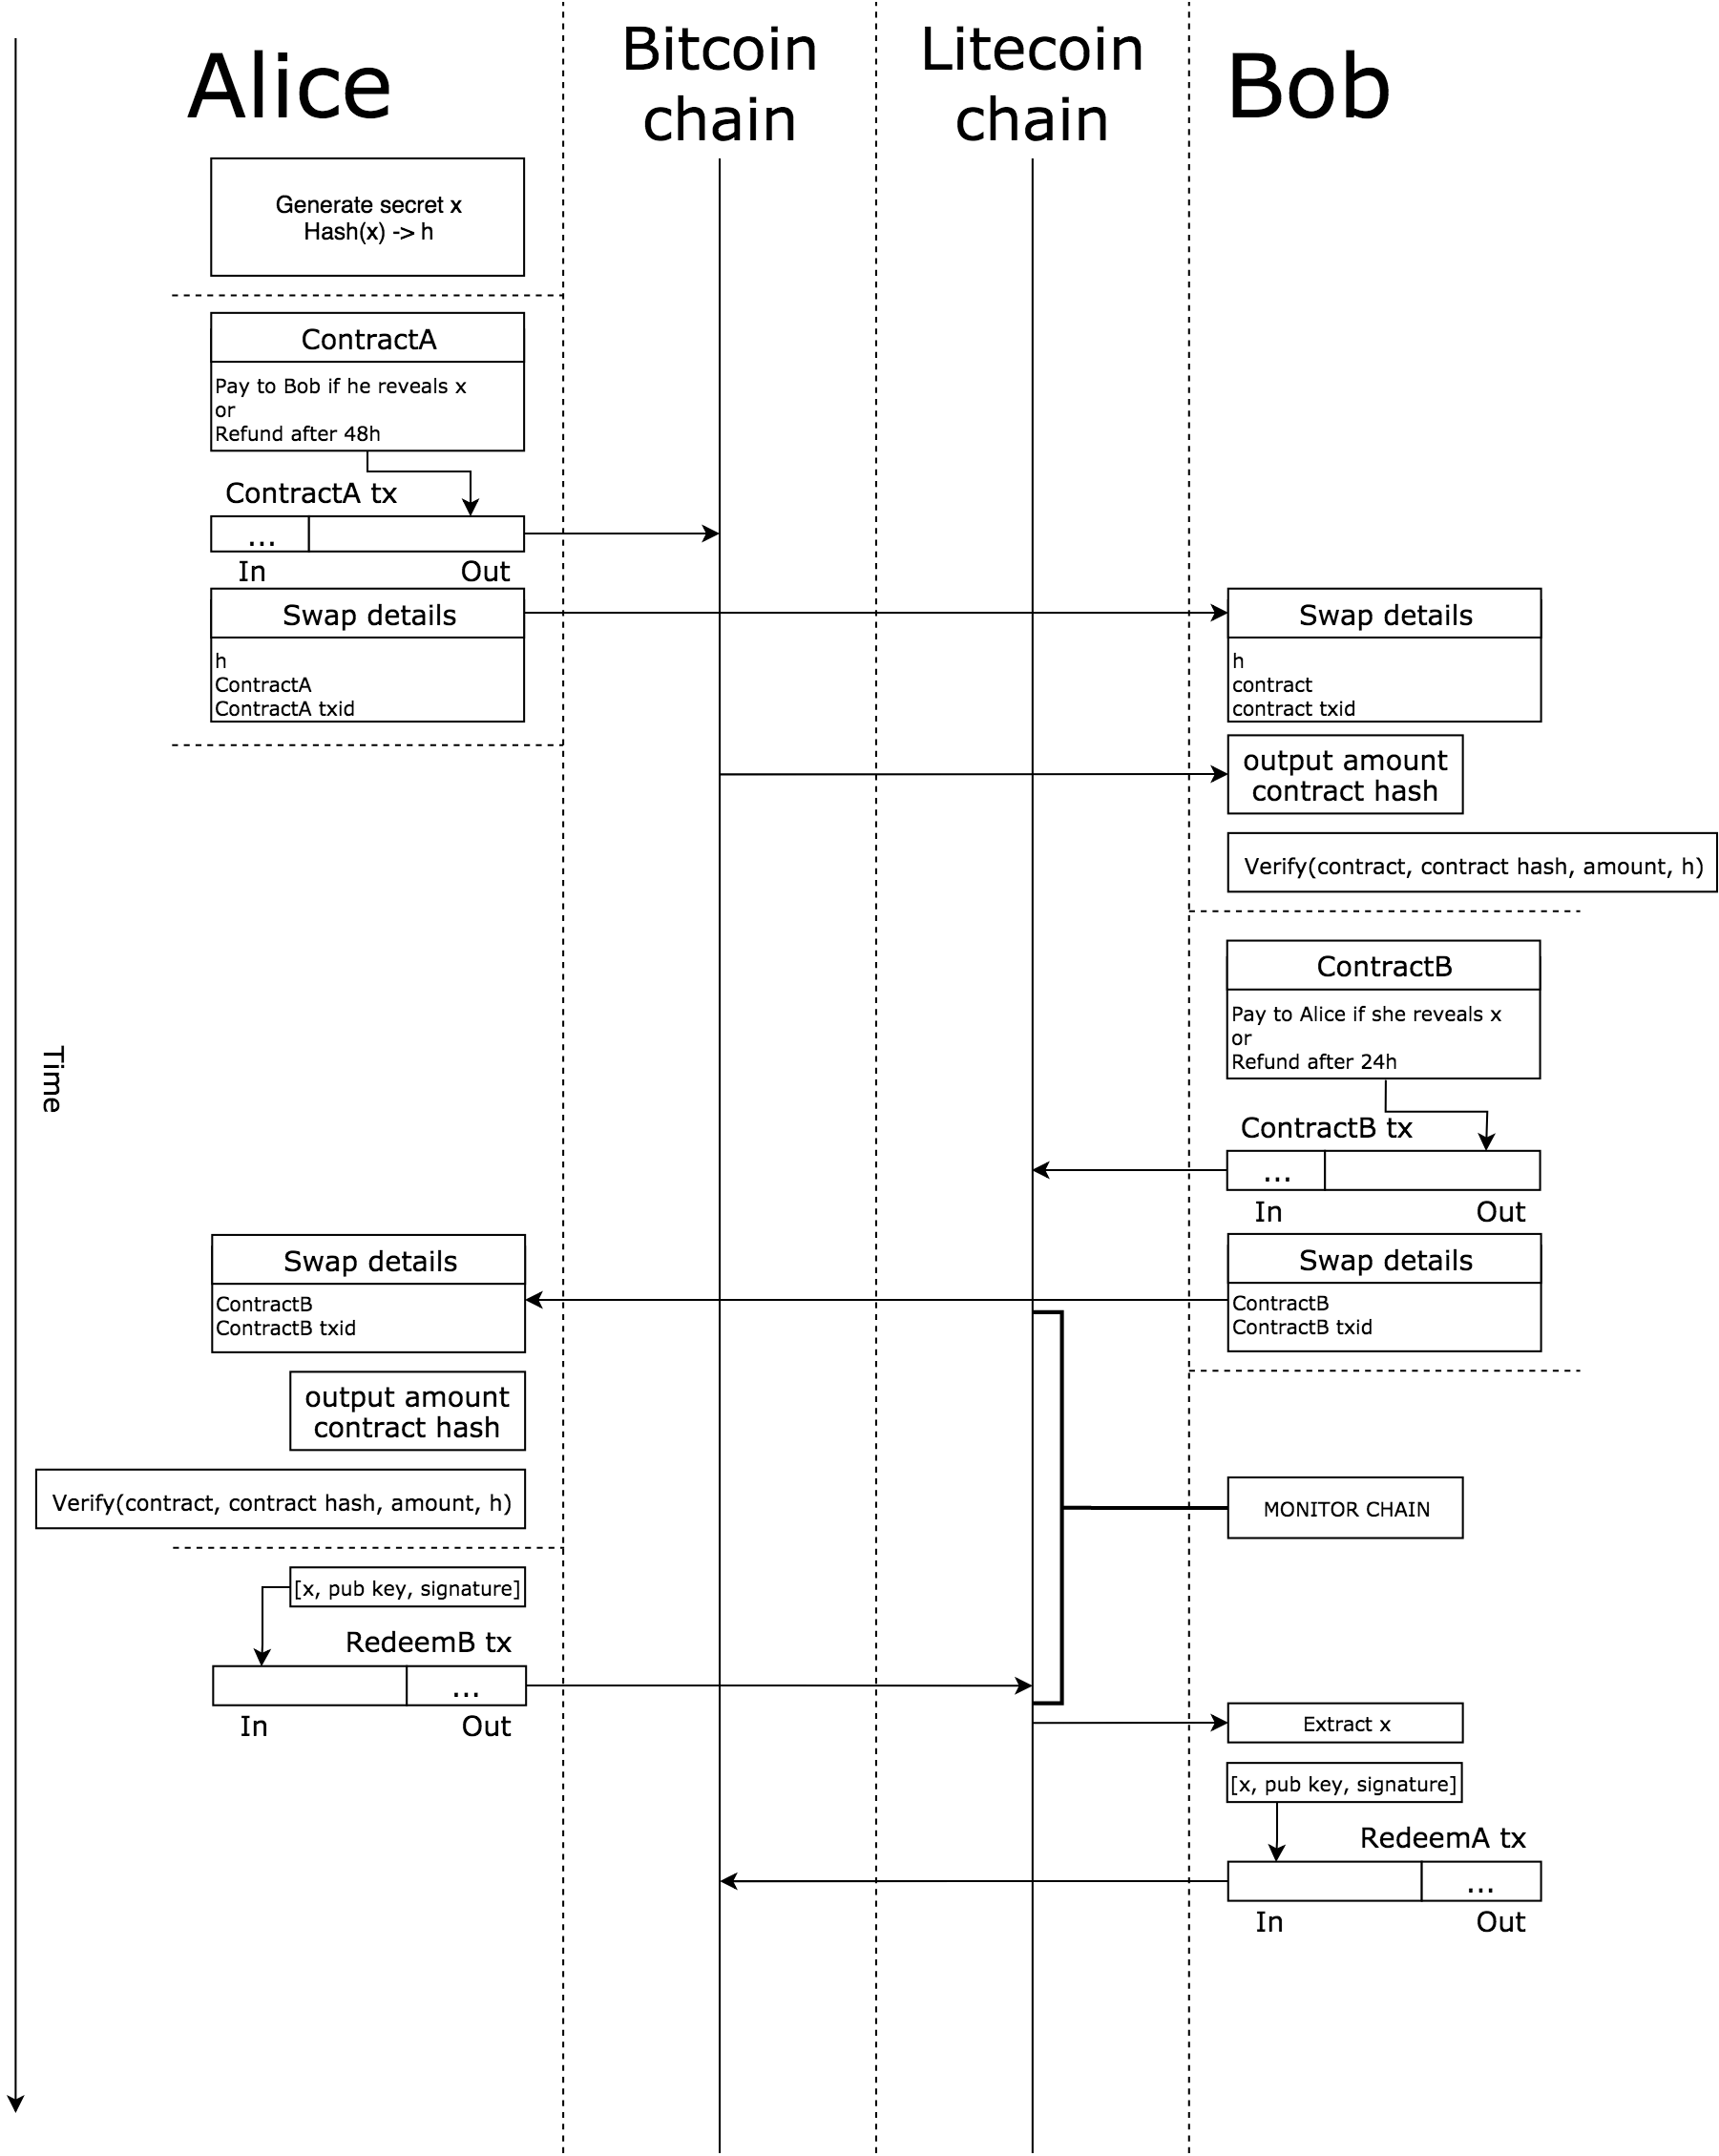
\includegraphics[width=1.35\textwidth]{background/images/atomic_swap_flow_large.png}}
\newpage

\Subsection{How the swap could fail}
The atomicity of the swap depends on each party acting rationally and not doing any mistakes that compromises the process. For example if Alice broadcasts her side of the contract and then reveals $x$ to Bob thorough some alternative communication channel then Bob could claim the Bitcoins without doing his part of the deal. 

Malformed contracts could also lead to money being stolen. This is why the validation steps are very important. For example Alice could maliciously set her contract to expire earlier than Bobs if Bob is not careful.

Actors in the scenario doing nothing also compromises the swap. If Alice waits til after $T/2$ expires before attempting to claim the Litecoins she is risking out on losing both the currencies. Bob could monitor the transaction pool, seeing what $x$ was, then sneak in his own refund transaction reclaiming his Litecoins (This is possible as the refund branch of the contract now is unlocked). Then also claiming the Bitcoins before $T$ expires.
\Section{Off-chain atomic swaps}
Atomic swaps over a payment channel is possible, often referred to as off-chain atomic swap. The mechanisms that makes it work may not be as clear as one that takes place entirely on-chain. 

To clear some things up before moving on: \textbf{both} parties that are performing the swap needs to have a functioning node on the respective networks of the cryptocurrencies to be exchanged. The channels do \textbf{not} need to be directly connected to each other instead they can take any route through both networks, given that the route allows the exchanged amount of course.

If we say that Alice (A) and Bob (B) want to do an off-chain atomic swap, Alice has bitcoins and wants litecoins, Bob has litecoins and wants bitcoins. Let us also say that Alice is the one that initiates the swap (meaning that in this case she sends the initial transaction). An off-chain atomic swap can be thought of as a transaction that propagates through both the networks. Alice sends a transaction to Bob on the bitcoin network, Bob re-sends a transaction with the same pre-image hash on the litecoin network to Alice. The timelocks are set so that the time continually decreases (like it would on a regular network transaction), even as it transitions into the litecoin network. Let us say that there are $m$ jumps between Alice and Bob on the bitcoin network and $n$ jumps between them on the litecoin network, and that each step needs at least 24 hours more to claim for each step. 

The timelock on the initial channel jump (the one Alice sends initially) would be:
$$(m+n+1) * 24h$$

When the transaction reaches Bob the timelock should be: 
$$(n+1) * 24h$$

This is where the swap differs from a normal transaction. In a regular transaction Bob would be the holder of the pre-image, and thus the pre-image could properly propagate backwards in the transaction chain from here. But in this case he does not know the pre-image and thus is forced to continue the chain on the litecoin side if he ever wants to claim his bitcoins. As mentioned he sends the agreed upon litecoins to Alice via the litecoin network, still using the same pre-image hash used by Alice. He also continues with the same decreasing timelock (thus the next transaction will have a timelock of ($(n+1 - 1) * 24h$)

When the transaction on the litecoin network at last arrives to Alice the timelock should be set to:
$$(1) * 24h$$

When the litecoin transaction reaches Alice the circle is closed and Alice can safely reveal the pre-image. Every one in the transaction chain gets their rightful money. When the pre-image reaches Bob he has to propagate it backwards on the bitcoin network until it reaches Alice again. Just as with regular multi-hop transactions each channel is expected to settle without closing and spending the HTLC-ouput unless necessary due to uncooperative nodes etc... 

As long as the same pre-image is used and the timelocks strictly decrease across the networks this should be a safe swap. If Bob tries to cheat Alice by not sending the agreed upon amount of litecoins Alice simply has to never reveal the pre-image anyone in the chain. Then all multi-hop transactions on both chains will have to be reset after the timelocks have expired.

\begin{figure}[H]
	\centering
	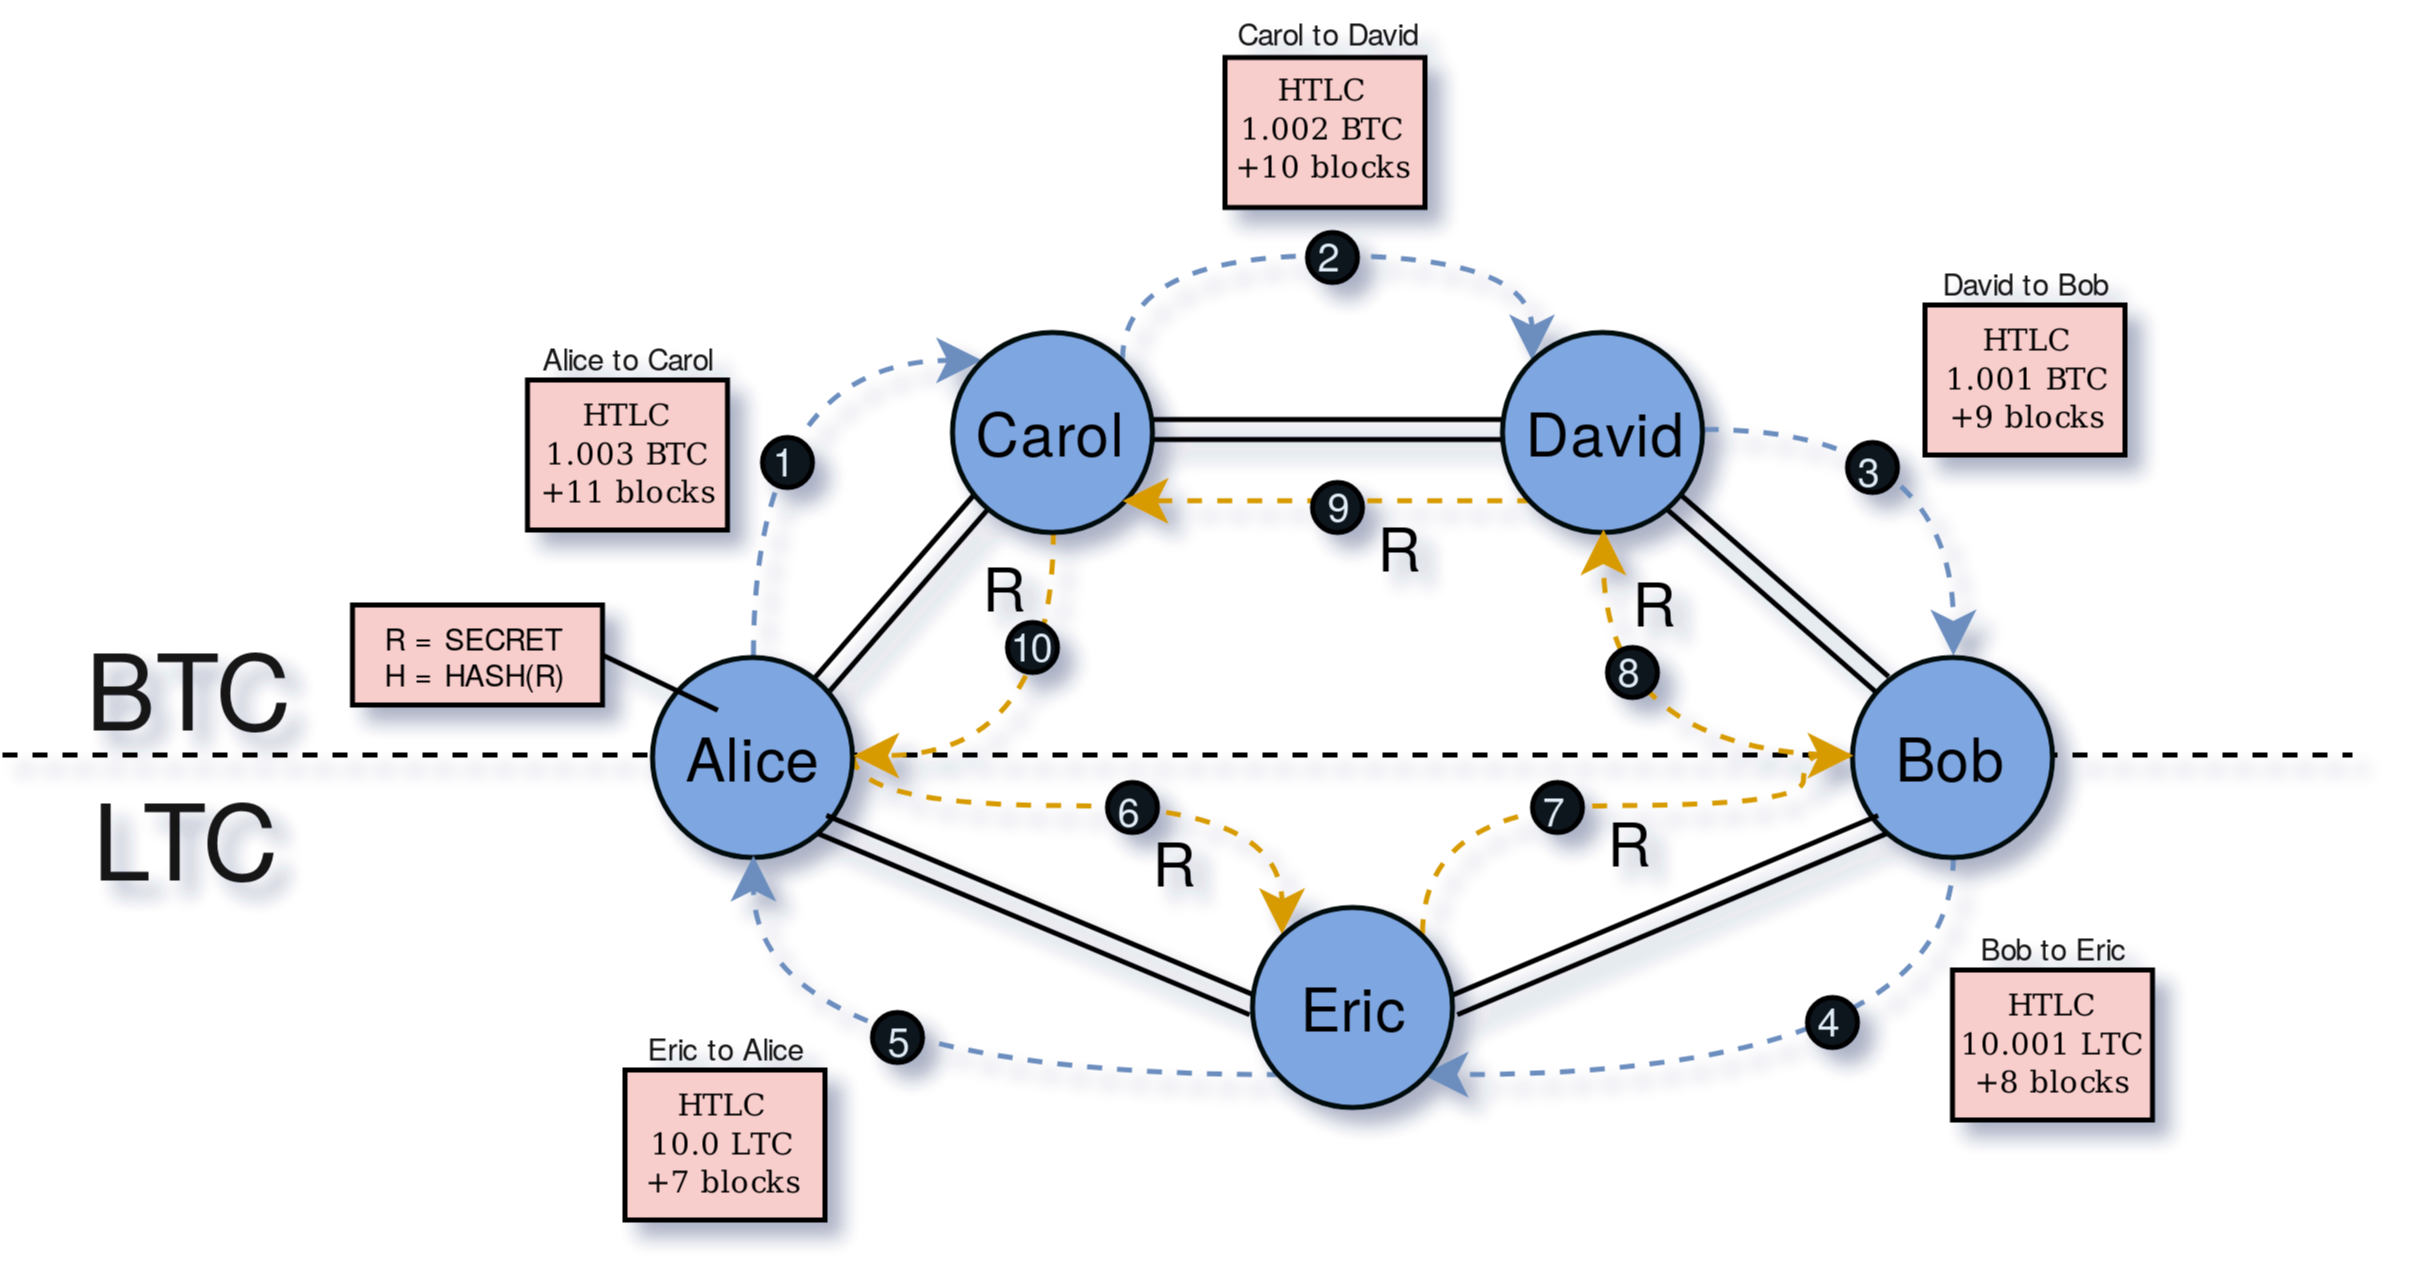
\includegraphics[width=1\textwidth]{background/images/ln_route_swap.png}
	\caption{Route taken by the multi-hop transactions on both networks. Note that Alice and Bob has a node in both the BTC and LTC network.}
	\label{fig:ln-swap}
\end{figure}

Figure \ref{fig:ln-swap} shows a rough diagram of the process. Alice and Bob has an active node in both the networks, no such assumption is needed for the other participants on either side. As mentioned the transaction could pass as many intermittent nodes as needed on either network, to keep the diagram small only two additional jumps are made on the Bitcoin side, and only one extra jump on the litecoin network.  

So to summarize the process: 

Alice and Bob agrees on doing a swap, they agree to exchange 1 bitcoin for 10 litecoins. Alice creates a new secret R and a new hash H = HASH(R). Sends an off-chain transaction to Bob on the bitcoin network that gives him 1 bitcoin if he can provide the pre-image to H (R) (Steps 1 - 3 in the diagram). Bob sends a multi-hop transaction to Alice on the litecoin network, that gives Alice 10 litecoins if she can provide the pre-image to H (Steps 4 - 5 in the diagram). It is very important that the decreasing timelock that was used on the bitcoin side continues on the litecoin side. Otherwise the safety of the swap is not guaranteed. 

When Alice receives the litecoin transaction, she can safely reveal R to Eric, Eric will do the same to Bob. The R will travel backwards in the transaction chain just like with a regular lightning network transaction, but this time when the pre-image reaches Bob he will keep transmitting it backwards through the chain on the bitcoin network. (Steps 6 - 10 in the diagram).

\Subsection{Safety}
The way safety is assured in off-chain atomic swaps is the same mechanisms that makes lightning network safe, which in turn is largely based on the mechanisms of the on-chain atomic swap. 
Let us take a look at a couple of scenarios where malicious actors try to claim money that is not theirs. Using the general scenario shown in figure \ref{fig:ln-swap}.

\Subsubsection{Bob does not send his litecoins to Alice after receiving bitcoins}
This would be after step 3 in the diagram. At first it may seem that Bob will get his bitcoins after all, but Alice simply has to never reveal the pre-image R. The HTLC contract states that everyone along the chain can only claim their money if they can reveal the pre-image to the hash H. If Alice never reveals it, Carol, David and Bob will not be able to claim the money. In the optimal case no channel will have to close in this scenario, after the timelock has expired nobody on the chain has any reason not to amend the previous commit with HTLC with a new commit with the transactions reversed. In the worst case, meaning that everybody refuses to cooperate, all the channels on the BTC side of the diagram has to be closed. The transaction reversal will be reflected on in the money that is now claimable on-chain.

In both the worst and best case no monetary loss has occurred for any of the participants in the network.

\Subsubsection{Alice tries to claim the litecoins without revealing the pre-image to Eric}
In this case she will be able to claim her litecoins. But claiming them on-chain will also reveal the secret R publicly on the blockchain. Even if Alice waited until just before the timelock expired to claim her litecoins, in this case 6 blocks, there is still time over for Eric to claim his litecoins on the Bob channel as that channel has a larger timelock. In the best case scenario only the channel between Alice and Eric is closed, while the rest settles normally (in this case in favor of the transaction). In the worst case all channels will have to be closed. Even so nobody will lose out on their share of the money as the timelock is ever increasing when going backwards in the payment chain, and for each step on the way the pre-image will be revealed on the blockchain just as it did between Alice and Eric. 

\Subsubsection{Somebody along the path stops cooperating}
Let us say Eric did not forward the transaction to Alice. This is just a variation of the first scenario. If Alice sees that something is wrong she will simply not reveal the pre-image to anyone and all channels will have to revert to previous state or be closed.

\chapter{Implementation}
To implement the described types of atomic swaps, Go (golang) was used together with the standard libraries plus external libraries from the \textbf{btcsuite}: \textbf{btcsuite/btcd} and \textbf{btcsuite/btcutil}, both of which can be found on github.com. The implementations are made to be simplified by design, focusing more on making it understandable for new-comers, and to save some time. The critical parts like actually 

\vspace{20mm}
More to come...


\chapter{Results \& Proposal}
\chapter{Discussion \& Future research}

\twocolumn


\onecolumn
% Bibliography
\bibliographystyle{plain}
\bibliography{reference}


\end{document}
